%%%%%%%%%%%%%%%%%%%%%%%%%%%%%%%%%%%%%%%%%%%%%%%%%%%%%%%%%%%%%%%%%%%%%%%%%%%%%%%
%                                                                             %
%           TEMPLATE LATEX PER TESI                                           %
%           ______________                                                    %
%                                                                             %
%           Ultima revisione: 11 Aprile 2025                                  %
%           Revisori: G.Presti; L.A.Ludovico; F. Avanzini; M. Tiraboschi      %
%                                                                             %
%%%%%%%%%%%%%%%%%%%%%%%%%%%%%%%%%%%%%%%%%%%%%%%%%%%%%%%%%%%%%%%%%%%%%%%%%%%%%%%
% Usare l'opzione twoside se volete stampare fronte-retro. Es.:
%\documentclass[twoside,12pt]{report}
% Si consiglia di diminuire il font per tesi di dottorato in formato 17x24. Es:
% \documentclass[11pt]{report}
\documentclass[12pt]{report}

% --- PREAMBOLO ---------------------------------------------------------------
% Inserire qui eventuali package da includere o 
% definizioni di comandi personalizzati

% Selezione lingua
\usepackage[italian]{babel}

\usepackage{tesi}
\lstdefinestyle{verbatim}{
    basicstyle=\ttfamily, % font style and size
    literate=
    *{\\}{{\textbackslash{}}}{1}, % \
}
\lstset{style=verbatim}
% Puoi usare il font di default di LaTeX con la relativa opzione del package
% \usepackage[defaultfont]{tesi}
% Esiste anche un'opzione per il formato 17x24 per le tesi di dottorato
% \usepackage[phd]{tesi}

% In caso il copia-incolla del PDF generato perda gli spazi,
% provare a decommentare la seguente riga
% \pdfinterwordspaceon

% !!! INFORMAZIONI SULLA TESI DA COMPILARE !!!

%   UNIVERSITA' E CORSO DI LAUREA:
\university{Università degli Studi di Milano}
\unilogo{immagini/loghi/unimi}
\faculty{Facoltà di Scienze e Tecnologie}
\department{Dipartimento di Informatica\\Giovanni Degli Antoni}
\cdl{Corso di Laurea Triennale in\\Sicurezza dei Sistemi e delle Reti Informatiche}

%   TITOLO TESI:
\title{Design e sviluppo di un tool per il Vulnerability Assesment di protocolli avanzati di rete}
% Questo comando (opzionale) sovrascrive \title per quanto riguarda la copertina
% Può essere usato per stampare caratteri speciali, tenendo i metadati puliti
\printedtitle{Design e sviluppo di un tool per il Vulnerability Assesment di protocolli avanzati di rete}

%   AUTORE:
\author{Falgiani Veronica}
\matricola{21191A}
% "Elaborato Finale" per i CdL triennali
% "Tesi di Laurea" per i CdL magistrali
\typeofthesis{ELABORATO FINALE}

%   RELATORE E CORRELATORE:
\relatore{Prof. Claudio A. ARDAGNA}
\correlatore{Prof. Nicola BENA}

%   LABORATORIO:
% Questa sezione crea una pagina di chiusura della tesi con
% il logo dell'ente/laboratorio presso cui si è svolto il tirocinio.
% Più afferenze/url/loghi sono supportate,
% e la frase può essere personalizzata.
% Qui trovate alcuni predefiniti del nostro dipartimento
% \adaptlab
% \aislab
% \anacletolab
% \bisplab
% \connetslab
% \everywarelab
% \falselab
% \iebilab
% \islab
% \lailalab
% \lalalab
% \lawlab
% \laserlab
% \limlab
% \mipslab
% \optlab
% \phuselab
% \ponglab
% \sesarlab
% \spdplab

% Esempio di personalizzazione della pagina di chiusura
% (non consegnate con questo esempio!)
% (da commentare in caso sia sufficiente una delle macro precedenti)
%\lab{Laboratorio di Ricerca}
%\lab[in collaborazione con l']{Azienda Specifica}
%\laburl{https://di.unimi.it/it/ricerca/risorse-e-luoghi-della-ricerca/laboratori-di-ricerca}
%\lablogo{immagini/redqmark}

% Con questo comando si può cambiare la dimensione (massima
% altezza e larghezza consentite) dei loghi
% \setlength\lablogosize{25mm}

%   ANNO ACCADEMICO
% \the\year inserisce l'anno corrente
% per specificare manualmente un anno accademico
% NON inserire nel formato 1970-1971, ma
% inserire solo 1970
\academicyear{2024} 

%   INDICI:
% elenco delle figure (facoltativo)
\figurespagetrue
% elenco delle tabelle (facoltativo)
\tablespagetrue
% prefazioni nell'indice (facoltativo)
% \prefaceintoctrue
% indice nell'indice (facoltativo)
% \tocintoctrue
% --- FINE PREAMBOLO ----------------------------------------------------------

\begin{document}

% Creazione automatica della copertina
% Centra la copertina nel foglio: usa questo comando per la copertina esterna
\makecenteredfrontpage
% Copertina allineata alle altre pagine: usa questo comando per la copertina interna
% \makefrontpage

\newpage 
\ % The empty page
\newpage

% 
%			PAGINA DI DEDICA E/O CITAZIONE
%			facoltativa, questa è l'unica cosa che dovete formattare a mano, un po' come vi pare
%

%{\raggedleft \large \sl Questa tesi è dedicata a...}
{\raggedleft \large \sl Ai miei genitori, per avermi supportata e incoraggiata con amore.\\A Roberto e alla sua famiglia, per avermi sempre accolto a braccia aperte.\\A tutte le persone che hanno lasciato un segno in questi 3 anni.\\}

\clearpage
\beforepreface

% 
%			PREFAZIONE (facoltativa)
%

%\prefacesection{Prefazione}


%
%			RINGRAZIAMENTI (facoltativi)
%

%\prefacesection{Ringraziamenti}

%
%			Creazione automatica dell'indice
%

\afterpreface

% 
%			CAPITOLO 1: Introduzione
% 

\chapter{Introduzione}

L'avvento di Internet ha portato grandi cambiamenti nella vita di tutti i giorni. Molte aziende hanno avuto la necessità di proporre i propri servizi sul web, per aumentare la portata e la comodità d'uso. Questa novità ha spinto le aziende alla creazione di grandi infrastrutture di rete per sopperire all'evoluzione digitale. Nella maggior parte dei casi una rete aziendale è composta da due elementi: una rete esterna "demilitarizzata" che offre i servizi al resto del mondo e una rete interna privata in cui sono connessi i dispositivi aziendali ed i server che forniscono dati alle applicazioni esposte all'esterno.

Queste due reti sono interconnesse tra loro, ma quella interna viene protetta da meccanismi di difesa avanzati, permettendo l'ingresso solo a chi è effettivamente autorizzato. Questo però non è sempre garantito, in quanto vulnerabilità presenti sulle macchine esterne potrebbero far evadere i controlli e concedere accessi indesiderati. Se le macchine interne dell'azienda sono a loro volta vulnerabili c'è la possibilità che un attaccante si insidi all'interno dei computer aziendali o peggio ancora acceda a database o informazioni sensibili. Se un malintenzionato riuscisse ad entrare in una rete interna vulnerabile sarebbe in grado di esfiltrare una grande mole di dati all'azienda, recando gravi danni economici ed alla reputazione.

Gli esperti di cybersicurezza sono in costante allerta per poter proteggere i sistemi di aziende e società da costanti minacce informatiche. Per fare ciò, come primo passo, è necessario verificare se i sistemi aziendali presentano versioni vulnerabili ad attacchi oppure configurazioni errate che portano a comportamenti indesiderati dei servizi. Questi controlli vengono fatti tramite un Vulnerability Assessment, una fase in cui vengono individuate le macchine che presentano o possono presentare falle di sicurezza. Svolgere tutto questo a mano richiederebbe troppo tempo e risorse, per questo molte aziende forniscono strumenti chiamati Vulnerability Scanner che compiono questa mansione in modo automatico. I risultati degli scanner non sempre sono completi o corretti, per questo sarà necessario testare a mano i risultati ottenuti -per poter verificare la presenza o meno delle vulnerabilità descritte nei report.\cite{scarfone2008technical}

I vulnerability scanner sono strumenti molto complessi e in costante aggiornamento, utilizzati di solito nelle prime fasi di un Penetration Testing. Inviando pacchetti ai servizi e analizzando le risposte è possibile scoprire nuove informazioni o sottolineare la presenza di vulnerabilità. Per fare ciò devono poter riconoscere e scambiare dati con una grossa mole di protocolli e servizi, necessitando un continuo aggiornamento. Questi scanner sono molto utili per facilitare e velocizzare l'individuazione di criticità all'interno della rete.

Il seguente elaborato si occuperà dello studio e dello sviluppo di un vulnerability scanner, cercando di proporre una soluzione alternativa a quelle già presenti sul mercato. L'obiettivo è la creazione di un applicativo altamente modulare e leggero, per poter essere facilmente personalizzato e installato sui dispositivi da monitorare. Un software del genere è molto complesso da sviluppare e di conseguenza si è scelto di implementare solo le funzionalità principali, ma rendendo il tutto facilmente modificabile per agevolare l'aggiunta di nuove feature.\\
Il documento è suddiviso nei seguenti capitoli:

Il \textbf{Capitolo 2} fornisce una descrizione degli strumenti già presenti sul mercato e ne analizza le funzionalità principali. 

Nel \textbf{Capitolo 3} vengono enunciati i principali protocolli della pila TCP/IP utilizzati all'interno del progetto, fornendone una breve descrizione.

Il \textbf{Capitolo 4} tratta l'analisi e la progettazione di un vulnerability scanner. Viene discusso innanzitutto il comportamento e le fasi di uno scanner, per poi trattare le tecnologie utilizzate.

Nel \textbf{Capitolo 5} viene trattata in dettaglio l'intera implementazione dell'applicativo, fornendo parti di codice e descrivendone il funzionamento.

Il \textbf{Capitolo 6} illustra la struttura dei file di test utilizzati dal software per poter verificare le vulnerabilità dei dispositivi.

Il \textbf{Capitolo 7} fornisce esempi sulle varie tipologie di file di risultati che vengono generati alla fine di una scansione.

Infine nel \textbf{Capitolo 8} vengono tratte le conclusioni e le criticità che potrebbero portare a sviluppi futuri dell'applicativo.

% 
%			CAPITOLO 2: Stato dell'Arte
% 

\chapter{Stato dell'arte}
\label{cap:introduzione}

Durante gli anni sono nati programmi di vulnerability assessment sempre più performanti e in continuo aggiornamento, per seguire l'avanzamento delle tecnologie e l'individuazione di nuove vulnerabilità. Un software molto accreditato e utilizzato commercialmente è Nessus, un vulnerability scanner che utilizza plug-in per svolgere test sui servizi in rete.

\'{E}  anche necessario citare due programmi che non sono inerentemente vulnerability scanner, ma presentano funzionalità affini: Nmap e Metasploit. Il primo è uno scanner di rete in grado di riconoscere porte aperte e servizi. Utilizza degli script per individuare vulnerabilità molto semplici e informazioni specifiche sui servizi individuati. Il secondo è un programma utilizzato per svolgere penetration testing e presenta dei moduli che permettono di compiere le fasi di reconaissance, footprinting, exploitation e post-exploitation. Le parti di questo software che sono di nostro interesse sono i moduli che svolgono scan di rete e individuazione di vulnerabilità.

Di seguito sono riportate informazioni più dettagliate riguardo ai programmi precedentemente descritti, in modo tale da fornire una visione d'insieme prima di trattare la soluzione proposta.

\section{Nessus}

Nessus\footnote{https://www.tenable.com/products/nessus} è un vulnerability scanner nato nel 1998 da parte di Tenable, una compagnia di cybersicurezza statunitense. Utilizza il paradigma client-server in quanto presenta un'interfaccia grafica in cui è possibile configurare la scansione e visualizzare i risultati (client), e un demone che svolge la scansione di host, porte, servizi e vulnerabilità (server).

Nell'interfaccia web è possibile selezionare dei template per svolgere scansioni di diverso genere, partendo da un semplice host discovery fino ad uno scan avanzato su servizi e configurazioni.
\begin{figure}[htbp]
	\centering
	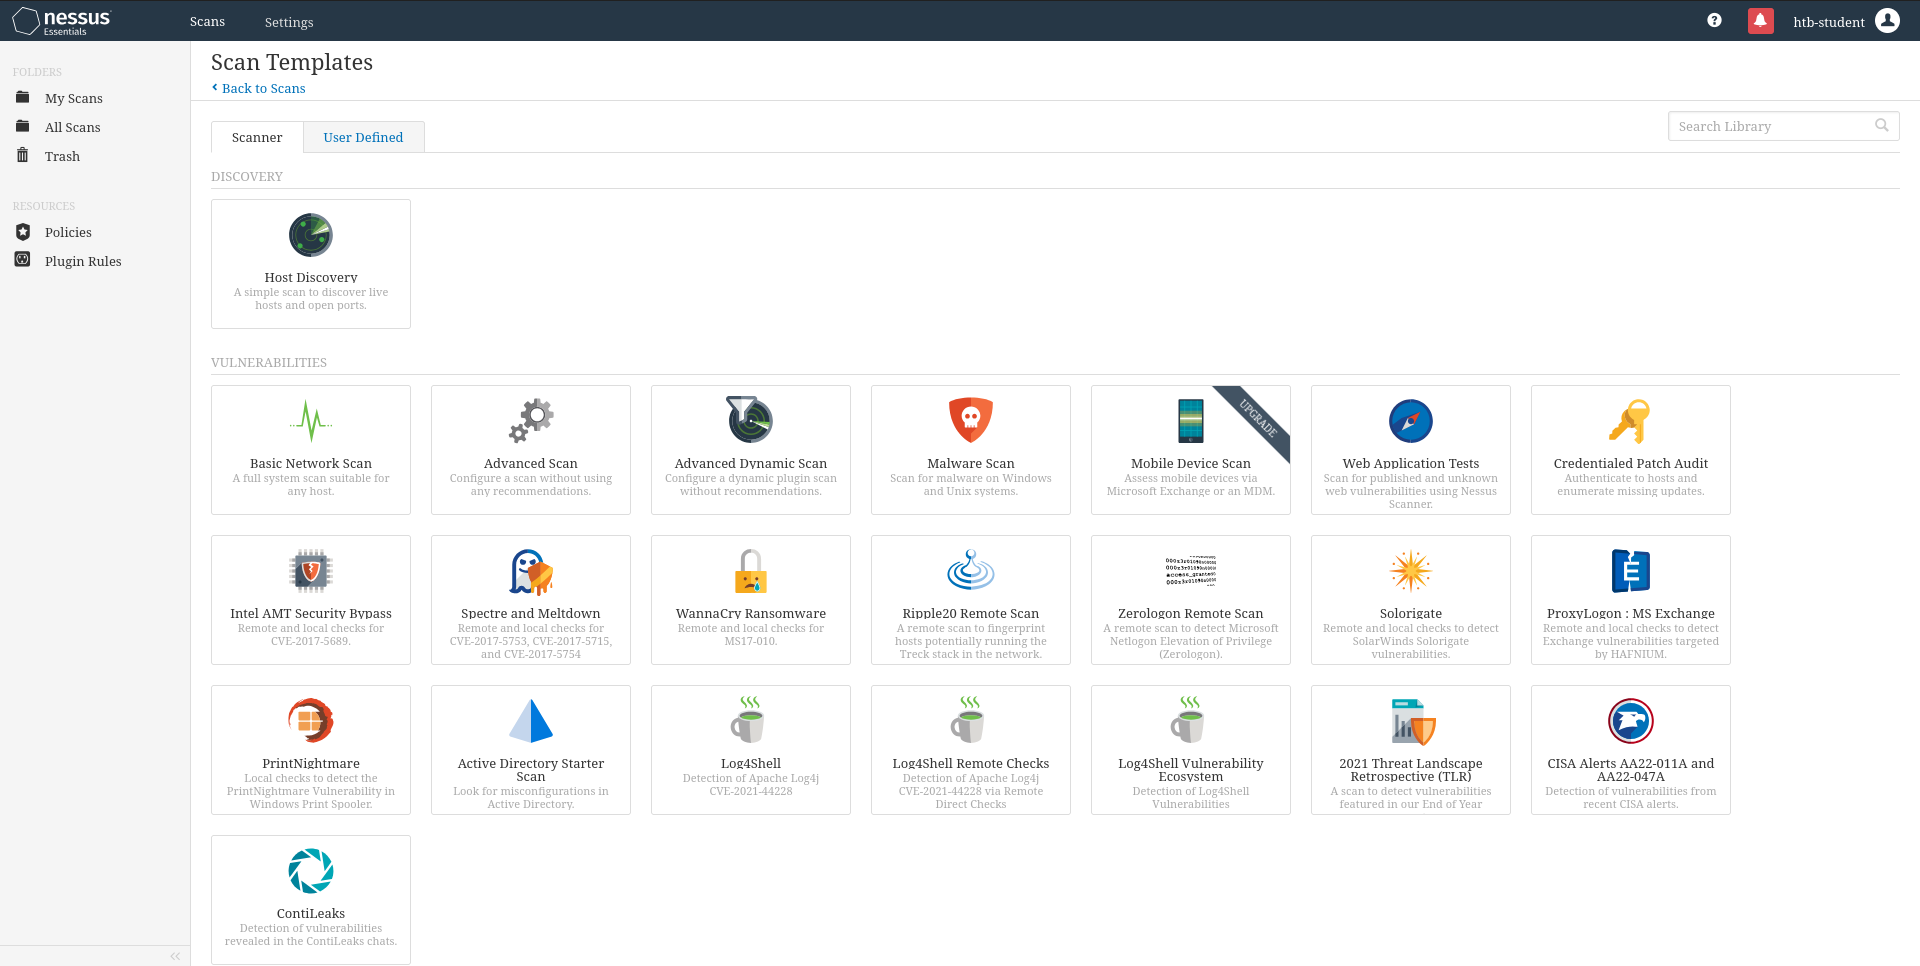
\includegraphics[width = 36em]{immagini/nessus.png}
	\caption{Lista di template per scansioni nell'interfaccia web di Nessus}
	\label{fig:nessus}
\end{figure}

Prima di iniziare lo scan vengono richieste informazioni sugli host e le modalità di svolgimento. \'{E} possibile scegliere l'aggressività dei test oppure abilitare delle opzioni per evadere i firewall e antivirus. Questo torna molto utile nelle scansioni in cui si vuole testare anche le prestazioni delle difese presenti nella rete.

Per svolgere il vulnearbility scan vengono utilizzati plug-in scritti tramite NASL (Nessus Attack Scripting Language), un linguaggio di programmazione creato appositamente per Nessus, che permettono di verificare la presenza di vulnerabilità o configurazioni errate all'interno dei servizi. Questi plug-in sono in continua crescita, per rimanere aggiornati sulle innumerevoli falle di sicurezza scoperte ogni giorno.

Una volta concluse le scansioni viene stilato un report che contiene gli host individuati. Per ogni dispositivo sono presenti una lista di vulnerabilità in ordine di gravità, che a loro volta contengono una descrizione, il CVE\footnote{https://www.cve.org/} di riferimento e le modalità per mitigarle. Successivamente i risultati possono essere esportati in vari formati, tra cui PDF, HTML, TXT e XML.

\begin{figure}[htbp]
	\centering
	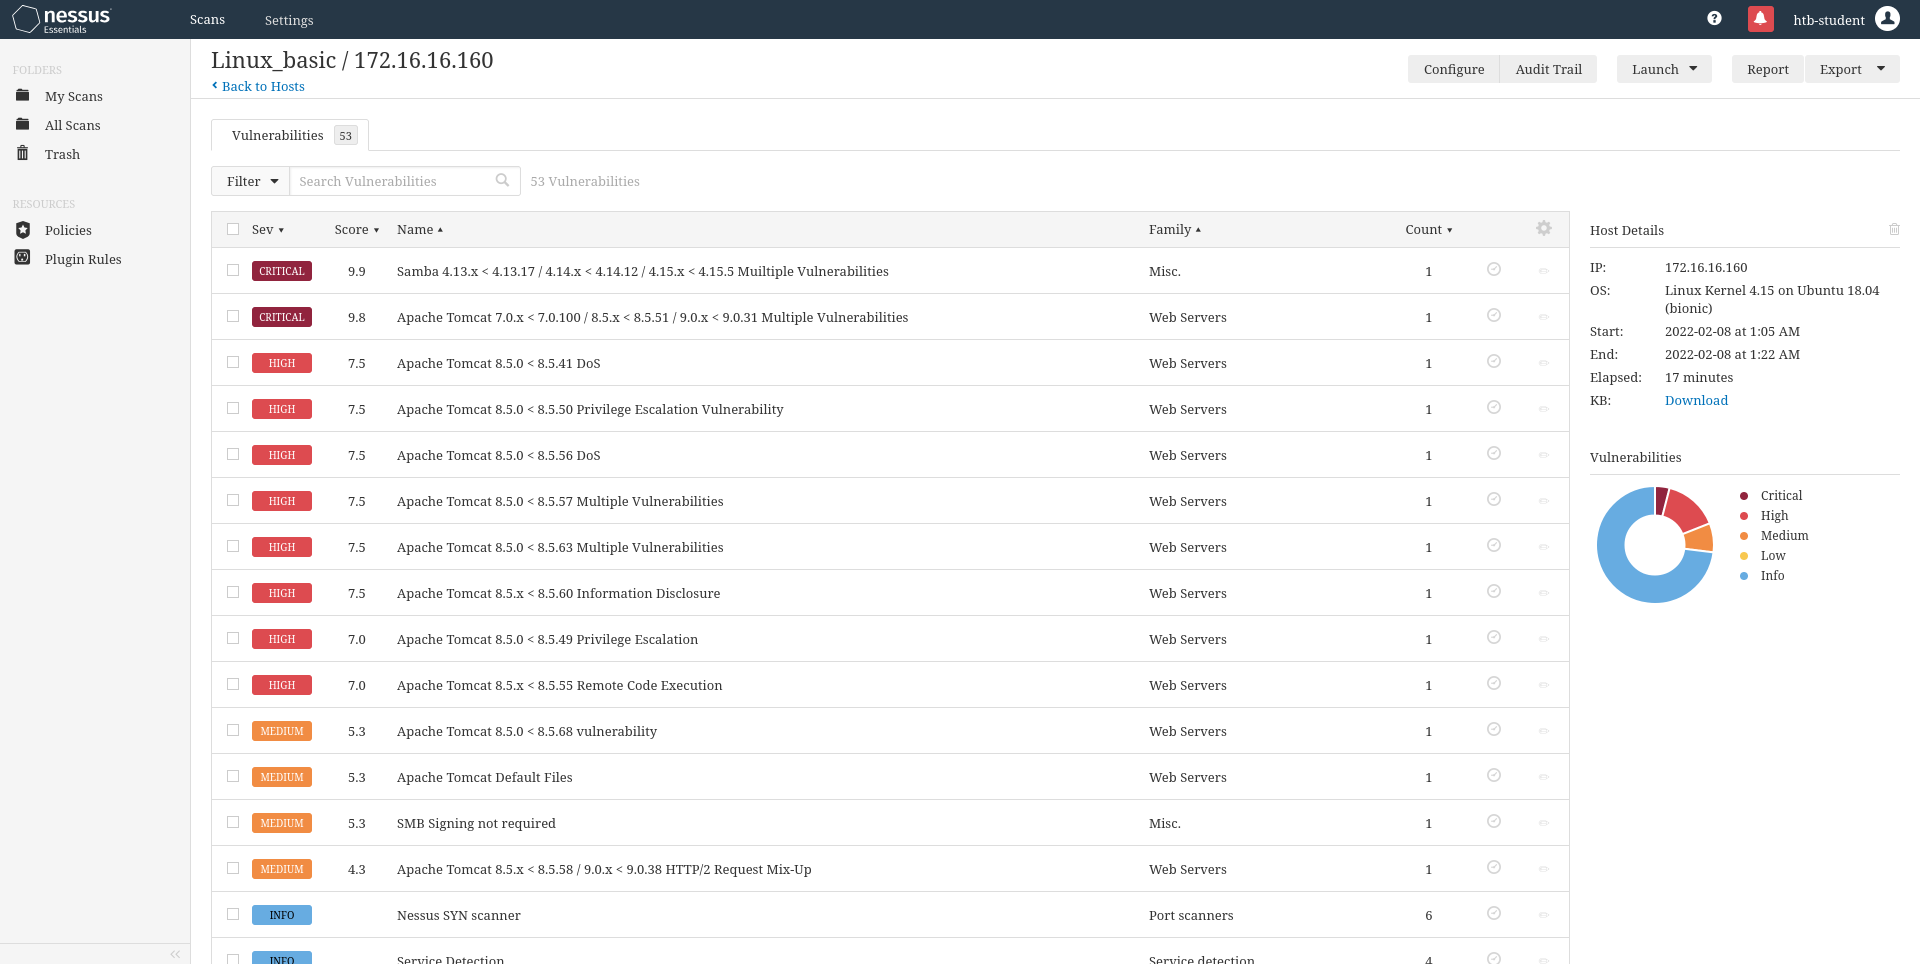
\includegraphics[width = 36em]{immagini/nessus_scan.png}
	\caption{Pagina dei risultati contenente le vulnerabilità presenti sull'host}
	\label{fig:nessus_scan}
\end{figure}

Nessus è diventato uno standard a livello professionale, ma sul mercato è anche presente un vulnerability scanner open source chiamato OpenVAS\footnote{Common Vulnerabilities and Exposures, https://www.openvas.org/}. Presenta le stesse funzionalità di Nessus, tra cui host discovery, network scan e vulnerabilty scan, ma è una valida alternativa per chi cerca software senza licenza a pagamento.

\section{Nmap}

Nmap\footnote{https://nmap.org/} è uno scanner di rete open source che permette la rilevazione di host attivi e il riconoscimento di porte aperte e servizi. \'{E} uno strumento che viene utilizzato esclusivamente da linea di comando (Zenmap è la versione che implementa una Graphical User Interface), ma permette il salvataggio dei risultati su file. Il funzionamento si basa sull'invio di pacchetti e la conseguente analisi delle risposte. 

Una scansione completa di Nmap si basa sulle seguenti fasi:
\begin{itemize}
    \item scoperta degli host: Nmap verifica se gli host sono attivi e raggiungibili inviando pacchetti e analizzando le informazioni contenute nella risposta. Sono presenti diverse modalità di scansione (ICMP, TCP-SYN, TCK-ACK, UDP...), ognuna utilizzata per svolgere analisi diverse, tra cui evasione di firewall o test delle difese nella rete.
    \item scansione delle porte: utilizzata per individuare quali porte sono aperte, filtrate (se è presente un dispositivo di difesa) o chiuse. Anche in questo caso Nmap può utilizzare modalità di scansioni differenti per ottenere risultati più precisi.
    \item scansione protocolli, servizi e sistema operativo: Nmap riconosce un protocollo quando all'invio di un pacchetto formattato secondo lo standard, riceve una risposta corretta che segue le regole stabilite dal protocollo stesso. 
    Se è stata richiesta l'individuazione dei servizi, vengono inviati dei "probe" verso le porte e le risposte sono comparate con un database contenente le relative firme e versioni. 
    Inoltre è possibile riconoscere il sistema operativo utilizzato andando ad analizzare bit per bit il contenuto di pacchetti TCP e UDP inviati. 
    \item esecuzione di script: il punto di forza di Nmap è l'NSE (Nmap Scripting Engine) che permette l'utilizzo di script per ampliare le funzionalità del network scanner, consentendo l'individuazione di informazioni dettagliate su servizi o testando la presenza di vulnerabilità. Non è paragonabile all'efficacia di un vulnerability scanner, ma può essere un ottimo indicatore di falle di sicurezza nelle fasi iniziali di scansione della rete.
\end{itemize}

Una volta terminate le scansioni i risultati vengono mostrati su linea di comando, ma utilizzando il parametro \lstinline{-o} è possibile salvarli all'interno di diverse tipologie di file. Il report finale mostra le porte, i protocolli utilizzati e i servizi presenti sull'host. Se sono stati utilizzati degli script viene anche riportato il risultato della loro esecuzione.

\begin{figure}[htbp]
	\centering
	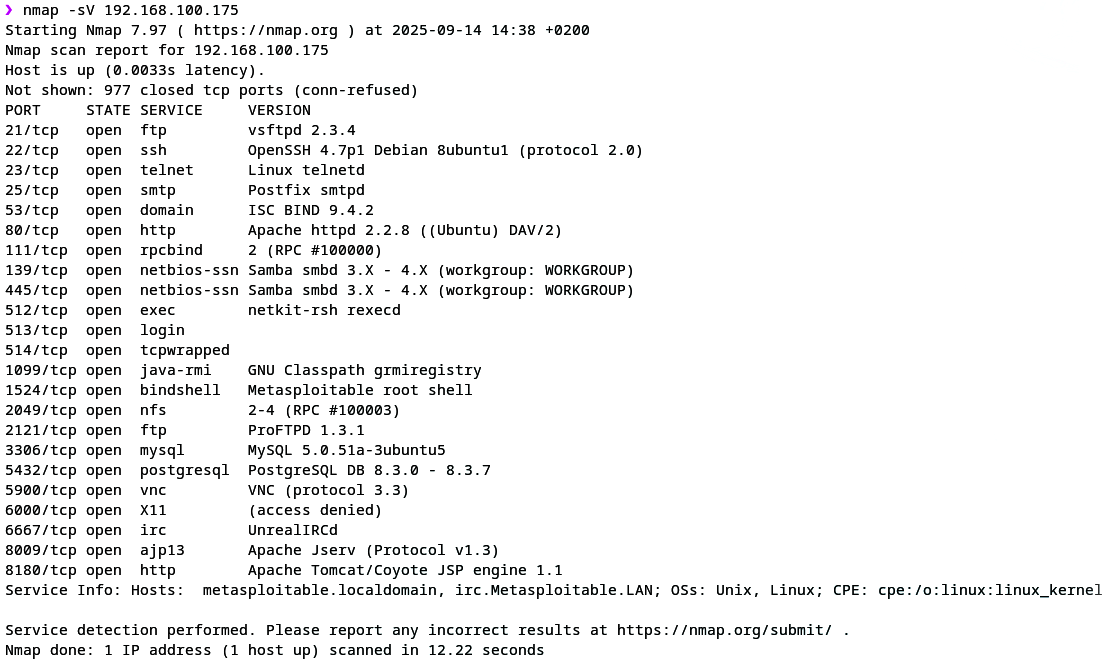
\includegraphics[width = 30em]{immagini/nmap_scan.png}
	\caption{Risultati della scansione tramite Nmap}
	\label{fig:metasploit}
\end{figure}

\section{Metasploit}

Metasploit\footnote{https://www.metasploit.com/} è un framework impiegato da esperti di cybersicurezza per svolgere penetration test. Tramite moduli sviluppati dalla comunità è in grado di compiere diverse operazioni, suddivise in:
\begin{itemize}
    \item auxiliary: script per analizzare, raccogliere, scansionare o testare DoS sulla macchina avversaria.
    \item encoder: utilizzati per codificare caratteri da inviare che potrebbero creare problemi.
    \item evasion: utili per manipolare payload e renderli difficilmente rilevabili da meccanismi di difesa.
    \item exploit: sfruttano vulnerabilità che permettono l'esecuzione di un payload sulla macchina compromessa
    \item nop: inviano una sequenza di "No Operation". Utilizzato in associazione con buffer overflow.
    \item payload: contengono shellcode utile da iniettare successivamente all'exploitation di un host.
    \item post: moduli utili per raccogliere ulteriori informazioni a seguito della manomissione di un host.
\end{itemize}

\begin{figure}[htbp]
	\centering
	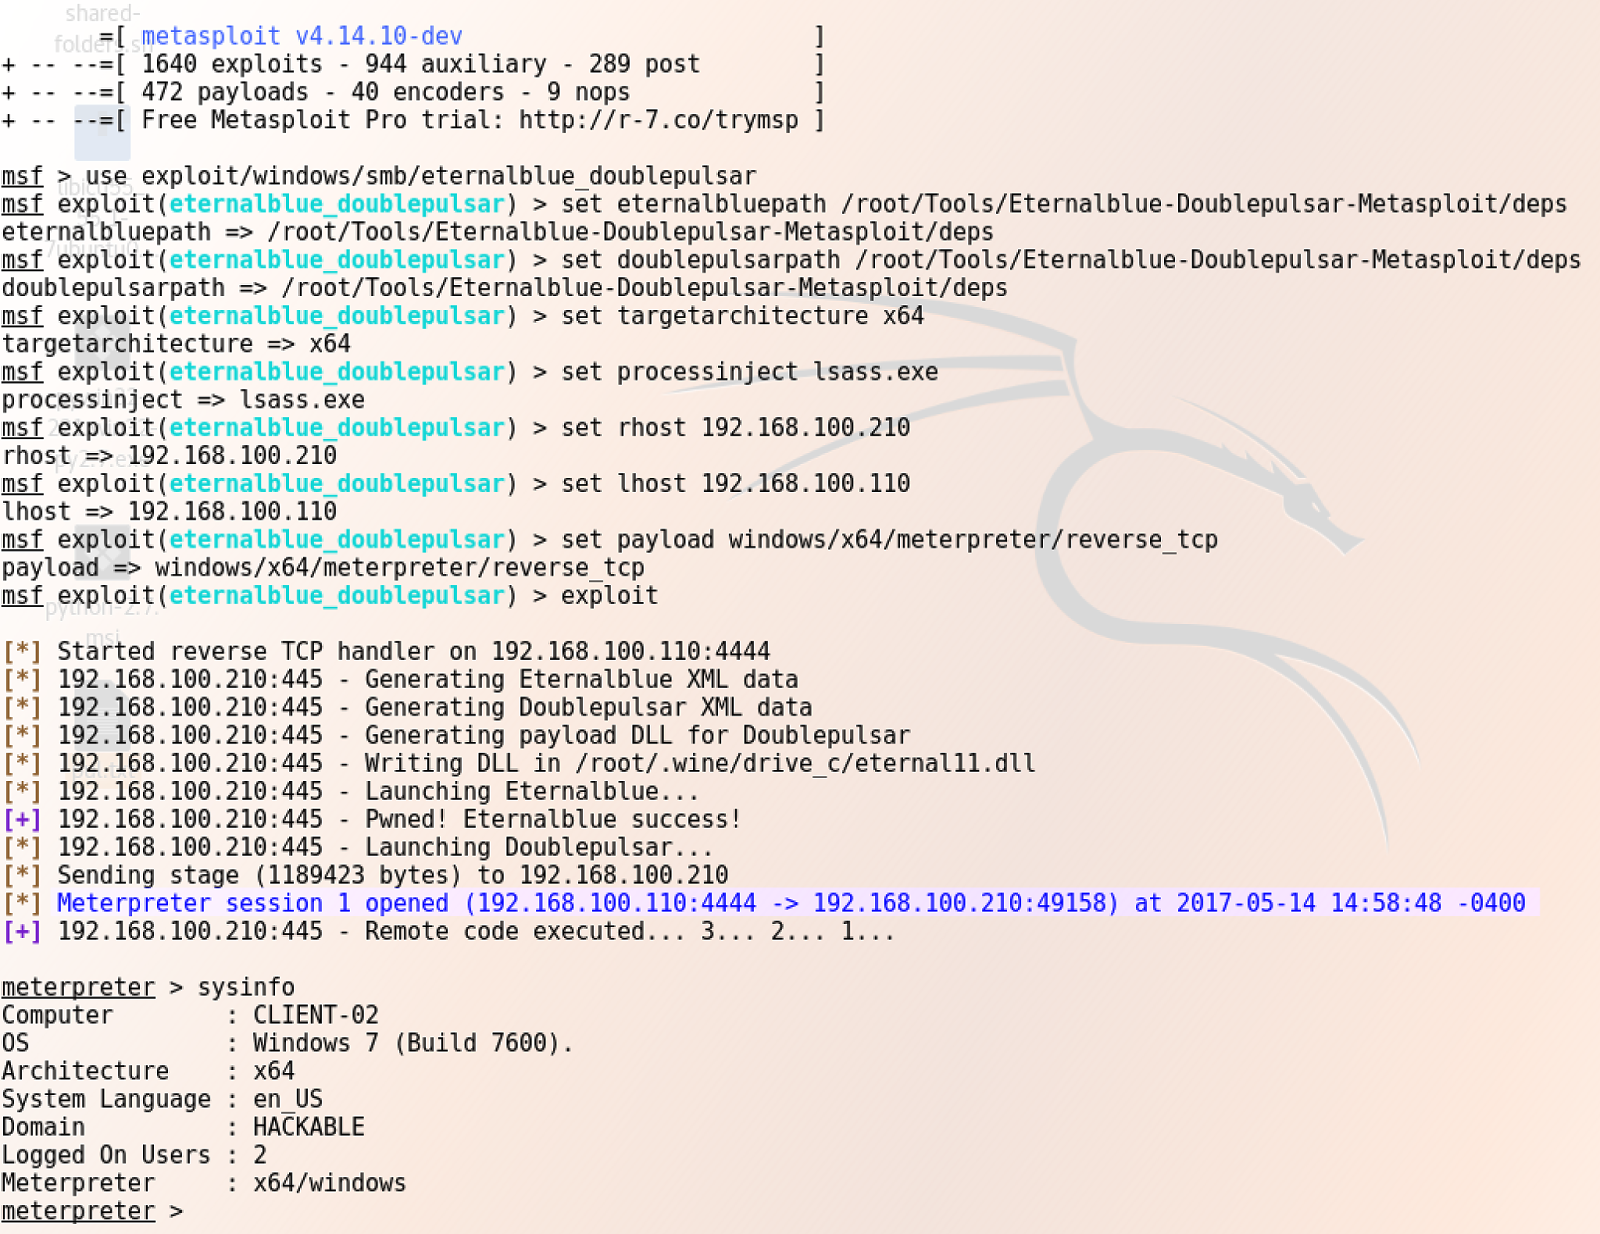
\includegraphics[width = 28em]{immagini/metasploit.png}
	\caption{Esempio di esecuzione di un modulo Metasploit}
	\label{fig:nmap}
\end{figure}

Il framework contiene strumenti aggiuntivi per poter ampliare le funzionalità e semplificarne l'utilizzo.
La console di Metasploit viene avviata da terminale tramite il comando \lstinline{msfconsole}. Questo strumento è utilizzato per interagire con il framework e per poter utilizzare i moduli. Per essere avviato è necessario richiamare \lstinline{msfconsole} da shell e, dopo un rapido caricamento, comparirà \lstinline{msf >}, indicandone il corretto avvio. Raggiunta questa schermata sarà possibile selezionare i moduli necessari per iniziare la fase di configurazione degli script, in cui verrà richiesta la compilazione di IP, porte, file, flag etc. Una volta inserite le informazioni il modulo potrà essere eseguito tramite \lstinline{run} e, una volta ultimato, verranno mostrati a schermo i risultati.

MSFdb è uno strumento di gestione di database e si basa su PostgreSQL. Permette l'importazione di scansioni da parte di scanner, come Nmap o Nessus, oppure l'esportazione di risultati ottenuti dai moduli di Metasploit. 

MsfVenom offre la possibilità di creare payload personalizzati per varie tipologie di target. Un punto di forza di questo strumento è la possibilità di codificarli utilizzando tecniche semplici o più avanzate. In questo modo il contenuto dei pacchetti inviati risulta meno sospetto agli occhi dei sistemi di difesa.

Meterpreter è un payload altamente avanzato e pieno di funzionalità che può essere installato all'interno della memoria della vittima. Oltre a stabilire una connessione con l'host, offre la possibilità di crittografare i pacchetti inviati, recuperare hash e manipolare i file all'interno del dispositivo. In generale è il payload utilizzato di default dagli exploit di metasploit.

L'ultima funzionalità trattata è Armitage, la GUI\footnote{Graphical User Interface} scritta in Java per poter interagire con il framework. A seguito di scansioni mostra, tramite un grafico, i collegamenti tra gli host di una rete. Per ogni dispositivo indica anche gli exploit che potrebbero essere utilizzati, oltre a fornire funzionalità per la navigazione di file e il recupero di hash.

Metasploit è uno strumento molto potente che può essere utilizzato anche per scopi illeciti. Molti attaccanti sfruttano le sue potenzialità per cercare di compromettere dispositivi e reti in tutto il mondo a scopo di lucro.

% 
%			CAPITOLO 3: Protocolli
% 

\chapter{Protocolli analizzati}
\label{cap:protocolli-analizzati}

Prima di analizzare le fasi di un vulnerablity scanner è buona cosa descrivere i protocolli alla base del suo funzionamento. Le reti di computer riescono a scambiarsi dati grazie ad uno standard chiamato Internet Protocol Suite, che definisce delle regole per poter comunicare tra host eterogenei. \'{E} composto da 4 livelli, ovvero Datalink, Internet, Trasporto e Applicazione, ma all'interno di questo progetto verranno trattati solamente gli ultimi tre. Per ogni livello sono presenti protocolli che svolgono funzioni diverse, che variano dalla semplice trasmissione dei pacchetti ad una gestione dei file condivisi sulla rete. Per motivi di complessità e tempo, nel progetto sono stati studiati e applicati i protocolli più utilizzati, partendo dai più semplici fino ad arrivare a protocolli più avanzati.\cite{computer2021tanenbaum}

\section{Protocolli Internet Layer}

Il secondo livello della pila TCP/IP è rappresentato dall'Internet layer. I protocolli, metodi e specifiche definti permettono l'instradamento di pacchetti tra host appartenenti a reti diverse. I  protocolli più utilizzati in questo livello sono l'IP e l'ICMP.
\\\\
\textbf{ICMP}
\\\\
L'Internet Control Message Protocol è principalmente utilizzato per l'invio di codici di stato per dare informazioni o indicare errori quando due dispositivi comunicano. Il suo scopo è quello di offrire uno strumento per diagnosticare e verificare lo stato dei computer connessi alla rete.\cite{rfcICMP}

Questo protocollo si basa sull'invio di "Control Messages", numeri che indicano degli stati ben definiti in cui si trova il sistema. Sono suddivisi in "Type", che definisce una categoria generica, e "Code", che rappresenta in modo dettagliato lo stato. Nello sviluppo di questo progetto viene tenuto conto di un numero ristretto di Control Messages, riportati nella tabella seguente:

\begin{table}[htbp]
\centering
\begin{tabular}{@{}lll@{}}
\toprule
\textbf{Type} & \textbf{Descrizione} & \textbf{Utilizzo} \\ \midrule
0 & Echo Reply & Risposta del server ad un echo request del client \\
3 & Destination Unreachable & Il server è spento o non è raggiungibile \\
8 & Echo Request & Client richiede lo stato del server \\ \bottomrule
\end{tabular}
\caption{Control Messages principali di ICMP}
\label{tab:ICMPType}
\end{table}

\section{Protocolli Transport Layer}

Il terzo livello della pila TCP/IP è rappresentato dal Transport Layer. I protocolli a livello di trasporto sono utilizzati per fornire un canale di comunicazione tra due host per l'invio di pacchetti. I due più utilizzati sono TCP(Transmission Control Protocol), che stabilisce una connessione affidabile, e UDP(User Datagram Protocol) che è rapido a discapito dell'inaffidabilità. 
\\\\
\textbf{TCP}
\\\\
Il Transmission Control Protocol è un protocollo orientato alla connessione che permette l'invio di pacchetti in modo affidabile ed ordinato. Viene utilizzato principalmente per l'invio di file, in quanto è necessario ricevere tutte le informazioni nella giusta sequenza per poterlo ricostruire in modo corretto. \cite{rfcTCP}

\begin{figure}[htbp]
	\centering
	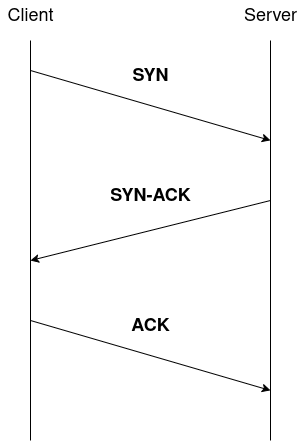
\includegraphics[width = 11em]{immagini/TCP3WH.drawio.png}
	\caption{Three-Way Handshake tra Client e Server}
	\label{fig:TCP3WH}
\end{figure}

All'interno dell'header di un pacchetto TCP sono presenti 8 bit detti "flags" che indicano lo stato della connessione. Questo è molto importante per svolgere l'operazione di "Three-Way Handshake", il processo per stabilire una connessione con l'interlocutore. Il Client ed il Server si scambiano rispettivamente le flag di SYN, SYN-ACK, ACK nella sequenza descritta, portando ad 1 i bit corrispondenti all'interno dell'header TCP. Nella figura \ref{fig:TCP3WH} viene illustrato il procedimento per l'apertura di una connessione TCP.

Oltre a queste flag, il protocollo TCP presenta altri valori che gli host si possono scambiare per ricevere maggiori informazioni sulla connessione. I principali utilizzati dal programma sviluppato sono:
\begin{itemize}
    \item URG: indica l'urgenza del pacchetto.
    \item ACK: notifica al mittente che il pacchetto è stato ricevuto correttamente,
    \item PSH: richiesta di spingere i dati nel buffer dell'applicazione ricevente.
    \item RST: resetta la connessione.
    \item SYN: utilizzato per stabilire una connessione 
    \item FIN: definisce l'ultimo pacchetto che il mittente vuole inviare prima della chiusura della connessione.
\end{itemize}
\textbf{UDP}
\\\\
Il protocollo UDP, a differenza di quello TCP, non è orientato alla connessione e di conseguenza la ricezione dei pacchetti non viene garantita. L'unità che viene inviata tra due host via UDP si chiama "datagramma". Gli utilizzi principali riguardano la trasmissione di dati in tempo reale poiché non è necessario ricevere tutti i pacchetti in modo ordinato. A discapito dell'affidabilità garantita da TCP tramite diversi controlli, UDP risulta molto più leggero e veloce.\cite{rfcUDP}

\section{Protocolli Application Layer}

L'ultimo livello della pila TCP è occupato dall'Application layer. \'{E} il livello che permette la comunicazione tra applicazioni presenti su due host differenti. Di conseguenza è il livello che contiene il maggior numero di protocolli. Ognuno si occupa di operazioni differenti, tra cui file sharing, gestione email, connessione a terminali remoti ecc.

In questa sezione i protocolli sono divisi in due categorie: protocolli semplici, che rappresentano i più utilizzati e i più facili da implementare, e i protocolli avanzati, che sfruttano meccanismi più complessi.

\subsection{Protocolli semplici}

\textbf{FTP}
\\\\
Il File Transfer Protocol permetto lo scambio di file da un dispositivo ad un altro. Ha un'architettura di tipo client-server e utilizza comandi predefiniti per permettere la comunicazione. Il server può richiedere al client un'autenticazione prima di svolgere delle operazioni. Se è abilitato si può eseguire il login tramite lo user "anonymous" e lasciando la password vuota.\cite{rfcFTP}

Una volta stabilita una connessione con il server si utilizzano i comandi descritti nella seguente tabella per comunicare.

\begin{table}[htbp]
\centering
\begin{tabular}{@{}m{4cm}m{10cm}@{}}
\toprule
\textbf{Comando} & \textbf{Descrizione} \\ \midrule
USER <username> & Inserire nome utente \\
PASS <password> & Inserire password dell'utente \\
PORT <host-port> & Specifica un indirizzo e una porta su cui il server dovrebbe connettersi \\ \bottomrule
\end{tabular}
\caption{Comandi principali di FTP}
\label{tab:FTP}
\end{table}
Il server utilizza codici di risposta per indicare il risultato dei comandi inviati:
\begin{itemize}
    \item 1xx e 3xx: errore
    \item 2xx: successo
    \item 4xx e 5xx: fallimento nel rispondere
\end{itemize}
\textbf{Telnet}
\\\\
Telent è un protocollo client-server basato su connessioni TCP che viene utilizzato per interagire con i terminali di dispositivi remoti. \'{E} stato deprecato per via di grossi problemi di sicurezza, tra cui la trasmissione in chiaro dei dati e la mancata autenticazione tra host. \cite{rfcTELNET}

Per poter interagire con terminali eterogenei tra loro Telenet utilizza il Network Virutal Terminal (NVT), un terminale virtuale che traduce i comandi nativi della macchina a comandi generici di Telnet. Una volta che client e server Telnet hanno stabilito una connessione, la comunicazione avviene tramite caratteri a 8 bit. Per inviare dati viene impostato il bit più significativo a 0 e i restanti bit vengono interpretati come caratteri ASCII. Per inviare comandi il bit più significativo viene impostato a 1. Telnet utilizza un'unica connessione per inviare dati e caratteri di controllo, ma all'interno dei messaggi, questi ultimi vengono preceduti da un carattere speciale chiamato Interpret as Control (IAC).  

\noindent
\textbf{SMTP}
\\\\
Il Simple Mail Transfer Protcol è utilizzato principalmente per il trasferimento di mail tra server di posta. Finita la composizione di una mail, l'host invierà il messaggio tramite il protocollo ad un primo server. Quest'ultimo a sua volta può passare il messaggio ad altri host finchè l'email non sarà recapitata al server di destinazione. Per poter scaricare le e-mail sul client sarà necessario utilizzare i protocolli POP e IMAP, che verranno trattati nelle sezioni successive.\cite{rfcSMTP}

I principali comandi utilizzati per la comunicazione sono i seguenti:
\begin{table}[htbp]
\centering
\begin{tabular}{@{}m{7cm}m{7cm}@{}}
\toprule
\textbf{Comando} & \textbf{Descrizione} \\ \midrule
HELO/EHLO & Permette di inizializzare la connessione tra due server \\ \hline
MAIL FROM <mittente@mail.com> & Inizializza il trasferimento di mail. \'{E} necessario specificare la mailbox del mittente da trasferire \\ \hline
RCPT TO <destinatario@mail.com & Specifica il destinatario. \'{E} possibile specificarne più di una mailbox \\ \hline
DATA & Tramite questo comando il client chiede al server di poter spedire i dati contenuti nelle mail. Una volta che il server avrà risposto positivamente, i messaggi verranno inviati riga per riga \\ \bottomrule
\end{tabular}
\caption{Comandi principali di SMTP}
\label{tab:comandi_SMTP}
\end{table}

In seguito all'invio di un messaggio ad un server, esso risponderà inviando un codice numerico che indica lo stato della transazione. Di seguito sono riportati i codici utilizzati con una piccola descrizione:
\begin{itemize}
    \item 2xx: operazione compiuta con successo
    \item 3xx: operazione intermedia compiuta con successo
    \item 4xx: errore temporaneo
    \item 5xx: errore permanente
\end{itemize}

\noindent
\textbf{DNS}
\\\\
Il Domain Name System consente l'assegnazione di nomi, detti anche nomi di dominio, agli host di una rete. 
Noi umani siamo molto più bravi a ricordarci nomi al posto di cifre e numeri. Per questo motivo si è voluto inventare un modo per poter assegnare dei nomi agli IP degli host. La traduzione da nome a IP è necessaria poiché i protocolli sottostanti hanno la necessità di utilizzare un indirizzo IP per poter funzionare secondo lo standard.\cite{rfcDNS}

Prima di passare al funzionamento del protocollo è buona cosa parlare della gerarchia dei server DNS. Se un client vuole collegarsi ad un sito web di cui conosce solo il nome di dominio e non il suo IP, sarà costretto ad interrogare il DNS resolver. Questo server è in grado di interagire con altri server DNS per poter recuperare le informazioni necessarie alla traduzione. Come primo passaggio il resolver interroga il Root DNS server, che fornisce l'indirizzo del Top Level Domain DNS server, ovvero colui che contiene i record per singoli TLD (per esempio .com o .net). Il resolver a questo punto interroga il TLD DNS server specificato precedentemente, che a sua volta restituisce l'indirizzo IP del nameserver autoritativo di dominio. A questo punto il resolver interroga come ultima cosa il server autoritativo che procoederà a restituire l'IP del server su cui si trova il servizio con il nome di dominio a cui il client voleva a accedere. A questo punto il resolver invia al client l'IP, con cui riuscirà a collegarsi al server.\cite{cloudflareDNS}

Ogni server DNS contiene al suo interno un database con campi che possono essere di diverso tipo. Di seguito sono riportati i più utilizzati:
\begin{table}[htbp]
\centering
\begin{tabular}{@{}m{3cm}m{11cm}@{}}
\toprule
\textbf{Tipo del campo} & \textbf{Descrizione} \\ \midrule
A e AAAA & Ritorna l'indirizzo IPv4 (A) oppure IPv6 (AAAA) di un host partendo dal suo nome \\ \hline
CNAME & Il nome di dominio specificato fa riferimento ad un altro nome \\ \hline
MX & Lista dei server che si occupano della ricezione di mail nel dominio \\ \hline
NS & Specifica il server autoritativo per il dominio specificato \\ \hline
SOA & Specifica le informazione del server DNS autoritativo, fornendo il name server primario, la mail dell'amministratore e altre informazioni \\ \hline
AXFR & Utilizzato per trasferire l'intero file della zona contente i record DNS tra un server DNS primario ed uno secondario \\ \bottomrule
\end{tabular}
\caption{Comandi principali di SMTP}
\label{tab:tipi_DNS}
\end{table}

Quando un client fa un richiesta ad un server viene inviato un messaggio che contiene al suo interno una query. Questa è composta da tre elementi: il nome, ovvero il nome di dominio che si vuole contattare, il tipo, cioè quale tipologia di campo DNS si vuole ricevere, e la classe, utilizzata per definire la classe del campo. Una volta ricevuta questa richiesta, il server risponderà a sua volta tramite un messaggio che contiene la risposta. All'interno possono esserci più elementi che descrivono tutti i record analizzati per arrivare all'IP desiderato. Ogni record presenta il nome, il tipo, la classe e in aggiunta dei dati, che a loro volta possono contenere un CNAME a cui fare riferimento oppure l'indirizzo IP stesso.

All'interno di un vulnerability scanner si cerca di fare una richiesta di tipo SOA verso le varie porte dei server per individuare quali utilizzano il protocollo. Se rispondono inviando informazioni sul server autoritativo c'è la certezza che la porta analizzata sia impiegata per le richieste e risposte di un DNS.
\\\\
\textbf{HTTP}
\\\\
L'HyperText Transfer Protocol è uno tra protocolli più utilizzati e permette lo scambio di informazioni tramite Internet. Durante gli anni sono state implementate diverse versioni, rispettivamente HTTP/1.0, HTTP/1.1, HTTP/2 e HTTP/3. Il protocollo implementa l'architettura client-server di tipo request-response. Questa tipologia funziona nel seguente modo: un host client invia una richiesta ad un server che elabora le informazioni per restituire una riposta. \cite{rfcHTTP}

Prima di analizzare i messaggi è necessario introdurre il concetto di metodi, header, body e codici di stato.

I metodi sono utilizzati all'interno delle richieste per specificare al server quale operazione si vuole svolgere su una risorsa. I metodi più utilizzati sono i seguenti:
\begin{table}[htbp]
\centering
\begin{tabular}{@{}m{3cm}m{11cm}@{}}
\toprule
\textbf{Tipo del campo} & \textbf{Descrizione} \\ \midrule
GET & Ricevere il dato indicato, senza apportare modifiche \\ \hline
POST & Inviare informazioni verso la risorsa specificata \\ \hline
PUT & Creare o modificare la risorsa specificata\\ \hline
DELETE & Eliminazione della risorsa specificata \\ \hline
HEAD & Restituisce gli header di risposta senza i contenuti del messaggio \\ \hline
OPTIONS & Descrive i metodi supportati dal server per la comunicazione \\ \bottomrule
\end{tabular}
\caption{Metodi di HTTP}
\label{tab:metodi_HTTP}
\end{table}

Gli header sono principalmente suddivisi in header di richiesta e header di risposta. Possono fornire informazioni aggiuntive sul messaggio inviato e gli host interessati, ma anche definire regole di sicurezza per limitare l'accesso di risorse a host non autorizzati. L'unico header obbligatorio all'interno di una richiesta HTTP è \lstinline{Host: www.example.com}, mentre i restanti possono essere omessi.

Il prossimo elemento da discutere è il body. Nelle richieste corrisponde alle informazioni o i dati che si vogliono comunicare al server per svolgere, ad esempio, un login o l'upload di un file. Nelle risposte invece contiene i dati della risorsa che è stata richiesta. Può essere una pagina web, uno script o addirittura un'immagine. 

Infine i codici di stato vengono utilizzati dal server per comunicare al client lo stato dell'elaborazione della richiesta. Sono rappresentati da numeri di 3 cifre, suddivisi in modo più generico in:
\begin{itemize}
    \item 1xx informational: invia informazione sullo stato delle operazione verso la specifica richiesta
    \item 2xx successful: l'operazione è andata a buon fine
    \item 3xx redirection: per completare la richiesta è necessario svolgere ulteriori operazioni
    \item 4xx client error: la richiesta è errata e non può essere soddisfatta
    \item 5xx server error: il server non è in grado di compiere l'operazione
\end{itemize}

A titolo d'esempio vengono mostrati i messaggi scambiati tramite protocollo HTTP/1.1.

\begin{lstlisting}[language=html, caption=Richiesta del client, basicstyle=\ttfamily\footnotesize, numbers=none]
GET / HTTP/1.1
Host: www.example.com
User-Agent: Mozilla/5.0
Accept: text/html,application/xhtml+xml,application/xml;q=0.9,image/avif,image/webp,*/*;q=0.8
Accept-Language: en-GB,en;q=0.5
Accept-Encoding: gzip, deflate, br
Connection: keep-alive
\end{lstlisting}

All'interno della richiesta sono presenti diversi elementi. Nella prima riga viene specificato il metodo di richiesta, il path della risorsa che si vuole accedere e la versione di HTTP che si vuole utilizzare. Le righe sottostanti sono composte dagli header della richiesta. Per quanto riguarda le richieste GET il messaggio dovrà terminare con due linee contenti i caratteri \lstinline{carriage return} e \lstinline{line feed}. Nelle richieste POST o PUT viene riportata solo una linea di terminazione, seguita dal contenuto dell'informazione che si vuole inviare al server.

\begin{lstlisting}[language=html, caption=Risposta del server, basicstyle=\ttfamily\footnotesize, numbers=none]
HTTP/1.1 200 OK
Date: Mon, 23 May 2005 22:38:34 GMT
Content-Type: text/html; charset=UTF-8
Content-Length: 155
Last-Modified: Wed, 08 Jan 2003 23:11:55 GMT
Server: Apache/1.3.3.7 (Unix) (Red-Hat/Linux)
ETag: "3f80f-1b6-3e1cb03b"
Accept-Ranges: bytes
Connection: close

<html>
  <head>
    <title>An Example Page</title>
  </head>
  <body>
    <p>Hello World, this is a very simple HTML document.</p>
  </body>
</html>
\end{lstlisting}

Nella prima riga della risposta è presente la versione di HTTP e il codice di stato a seguito dell'operazione. Nelle righe sottostanti sono riportati gli header di risposta e, dopo una linea contenente \lstinline{carriage return} e \lstinline{line feed}, viene riportata la risorsa richiesta.\cite{rfcHTTPSEMANTIC}
\\\\
\textbf{POP}
\\\\
Il Post Office Protocol viene utilizzato per recuperare, tramite un client, le e-mail presenti su un mail server. La versione più recente che viene utilizzata è la POP3. Questo protocollo, una volta collegato al server di posta, scarica tutte le e-mail presenti e le salva sul client. Successivamente le elimina definitivamente dal server. Questo metodo per scaricare la posta è un approccio che non rispecchia le necessità moderne di poter accedere alle medesime risorse da diversi dispositivi. Per questo è stato implementato il protocollo IMAP, discusso nella sezione successiva.\cite{rfcPOP}

Per poter comunicare con il server di posta remoto, l'utente deve autenticarsi e successivamente utilizzare una serie di comandi per comunicare.
\begin{table}[htbp]
\centering
\begin{tabular}{@{}m{3cm}m{11cm}@{}}
\toprule
\textbf{Tipo del campo} & \textbf{Descrizione} \\ \midrule
STAT & Mostra il numero di messaggi di una mailbox \\ \hline
LIST & Ritorna la lista di messaggi nella mailbox \\ \hline
RETR & Recupera il messaggio specificato \\ \hline
DELE & Elimina il messaggio dal server, di solito dopo che l'utente l'ha scaricato in locale \\ \bottomrule
\end{tabular}
\caption{Comandi POP3}
\label{tab:comandi_POP3}
\end{table}

\newpage
\noindent
\textbf{IMAP}
\\\\
L'Internet Message Access Protocol viene utilizzato per recuperare le mail da un server di posta. A differenza del protocollo POP3, il client scarica una copia delle mail presenti sul server, in modo tale da poterle visionarle su più dispositivi. Le modifiche apportate alla casella di un client vengono rispecchiate su tutti i restanti dispositivi. \cite{rfcIMAP}

La comunicazione tra client e server avviene tramite l'utilizzo di comandi.
\begin{table}[htbp]
\centering
\begin{tabular}{@{}m{3cm}m{11cm}@{}}
\toprule
\textbf{Tipo del campo} & \textbf{Descrizione} \\ \midrule
SELECT & Specifica a quale mailbox accedere \\ \hline
EXAMINE & Accede alla mailbox in modalità solo lettura \\ \hline
LIST & Mostra le cartelle presenti nella mailbox \\ \hline
FETCH & Recupera il contenuto delle e-mail \\ \bottomrule
\end{tabular}
\caption{Comandi IMAP}
\label{tab:comandi_IMAP}
\end{table}

\noindent
\textbf{SMB}
\\\\
Il Server Message Block è un protocollo utilizzato per la condivisione di file attraverso dispositivi presenti sulla rete. I principali dialetti SMB sviluppati nel corso degli anni sono: SMB1, CIFS, SMB2 e SMB3.\cite{microsoftSMB}

Anche in questo caso la comunicazione è di tipo client-server. Per poter accedere ad una risorsa è necessario compiere i seguenti passaggi, portati a termine inviando pacchetti formattati secondo lo standard SMB:
\begin{itemize}
    \item Stabilire una connessione tra client e sever tramite l'utilizzo di NetBIOS, un protocollo che permette la comunicazione tra dispositivi appartenenti alla stessa LAN.
    \item Negoziazione del dialetto di SMB che si vuole utilizzare. Il pacchetto inviato in questo passaggio è \lstinline{SMB_COM_NEGOTIATE}
    \item Il client svolge l'autenticazione verso il server.
    \item Connessione del client verso una share del server, ovvero una cartella condivisa. La richiesta viene portata a termine tramite il pacchetto \lstinline{SMB_COM_TREE_CONNECT_ANDX}
    \item Il client ora è in grado di aprire e leggere i contenuti dei file presenti sulla share del server. I pacchetti utilizzati per svolgere queste due operazioni sono \lstinline{SMB_COM_OPEN_ANDX} e \lstinline{SMB_COM_READ_ANDX}
\end{itemize}

\subsection{Protocolli avanzati}

\textbf{SSH}
\\\\
Il Secure Shell è un protocollo crittografico per svolgere operazioni su dispositivi presenti sulla rete. \'{E} stato sviluppato per sostituire i protocolli Telnet e Remote Shell per via delle loro comunicazioni non crittografate.

Come già accennato SSH utilizza crittografia a chiave pubblica per autenticarsi verso gli host remoti. L'autenticazione dell'utente può avvenire in due principali modalità: tramite password oppure publickey. Nella prima il protocollo genera automaticamente una coppia di chiavi e poi richiede all'utente una password. Nella seconda l'utente genera una coppia di chiavi che lo autentica automaticamente. Per potersi collegare ai dispositivi senza usare la password sarà necessario inserire la chiave privata al loro interno.

Il protocollo secure shell permette anche di svolgere diverse operazioni, rendendo obsoleti vecchi protocolli. Oltre alla possibilità di fare login su host della rete permette anche il trasferimento di file, il tunneling, il port forwarding e molto altro.\cite{rfcSSH}

L'architettura di SSH è suddivisa in tre livelli:
\begin{itemize}
    \item Transport layer: gestisce lo scambio di chiavi, l'autenticazione con il server e la crittografia del canale.
    \item Authentication layer: gestisce l'autenticazione tramite un gran numero di algoritmi. Il dispositivo client sarà sempre il primo a richiedere l'autenticazione al server.
    \item Connection layer: ogni connessione SSH può essere suddivisa e gestita su più canali che sono in grado di scambiare dati in modo bidirezionale.
\end{itemize}

\noindent
\textbf{MQTT}
\\\\
Message Queuing Telemetry Transport è un protocollo leggero di tipo publish-subscribe utilizzato soprattutto sui dispositivi dell'Internet of Things. 

L'MQTT definisce due dispositivi distinti: il broker e il client. I client per poter comunicare con i broker devono fare il \lstinline{subscribe} a dei "Topic". Successivamente possono inviare i messaggi usando il comando \lstinline{publish}, che invia al broker messaggi aventi un Topic associato. A questo punto il broker funge da intermediario, indirizzando i messaggi in base al loro Topic verso tutti i dispositivi sottoscritti. I client possono anche ricevere configurazioni o comandi data la bidirezionalità dal canale di comunicazione.\cite{oasisMQTT}
\\\\
\textbf{NFS}
\\\\
Il Network File System permette agli utenti di un computer di accedere a file condivisi sulla rete. Il protocollo si articola in 3 versioni differenti: NSFv2, NFSv3 e NFSv4. La comunicazione tra client e server avviene tramite l'utilizzo di Remote Procedure Call che servono per richiamare subroutine su un altro dispositivo.\cite{rfcNFS}

Per poter interagire con i file presenti sulla rete, il client ed il server devono svolgere i seguenti passaggi:\cite{eventhelixNFS}
\begin{itemize}
    \item Il server presenta tre servizi: il port mapper, mountd daemon e NFSD daemon. Il port mapper rimane in ascolto sulle porte 1111 UDP e TCP. NFSD e mountd richiedono al port mapper di registrare il numero delle porte su cui operare.
    \item Il client a questo punto richiede di montare il filesystem presente sul server. Il servizio di port mapping restituisce al client la porta su cui risiede il servizio mountd
    \item A questo punto il client richiede a mountd di poter montare il filesystem. Il server lo autentica e svolge l'operazione di montaggio. Al termine comunica al client i risultati dell'operazione. 
    \item Per poter svolgere operazioni di lettura e scrittura il client richiede al mapper la porta su cui risiede il servizio NFSD. Una volta restituito il valore, il client potrà svolgere operazioni di lettura e scrittura sul file system montato.
\end{itemize}

\noindent
\textbf{SSL/TLS}
\\\\
Il Secure Socket Layer e il Transport Layer Security sono dei protocolli crittografici che offrono la possibilità di cifrare comunicazioni attraverso la rete.\cite{rfcTLS} Il protocollo SSL ha avuto 3 versioni, ma è stato deprecato a favore delle varianti TLS1.2 e TLS1.3 che sono molto più sicure.\cite{rfcSSLDEP} Questi protocolli offrono anche la possibilità di autenticazione grazie all'utilizzo di certificati stipulati tra due o più applicazioni che vogliono comunicare.

Per poter rendere sicura una connessione è necessario l'utilizzo di un certificato digitale. Questi sono utilizzati per associare un'identità ad una chiave pubblica e vengono rilasciati da Certification Authority. Il TLS ha un legame di fiducia verso alcuni CA di terze parti che utilizza per verificare l'autenticità dei certificati utilizzati.\cite{ChadwickDavidW2001ETia}

Per iniziare una connessione sicura il client ed il server devono svolgere le seguenti operazioni:
\begin{itemize}
    \item Il client si connette ad una porta su cui è possibile iniziare una connessione sicura. Invia al server una lista che contiene tutti i cifrari che supporta.
    \item Il server a questo punto invia un messaggio al client specificando il cifrario scelto. Inoltre invia il certificato digitale per identificarsi.
    \item Il client verifica la correttezza dei dati e la validità del certificato.
    \item Successivamente il client deve creare una chiave di sessione cifrando un numero casuale oppure utilizzando lo scambio di chiavi Diffie-Hellman.
    \item Una volta portate a termine queste operazioni verrà inizializzata la connessione sicura.
\end{itemize}

% 
%			CAPITOLO 4: Progettazione
% 

\chapter{Progettazione}
\label{cap:progettazione}

I programmi precedentemente citati nello Stato dell'Arte sono molto complessi ed avanzati, con una curva di apprendimento abbastanza ripida. Per poter utilizzare un vulnerability scanner è necessario inizialmente scaricare una grande mole di dati e informazioni per poter svolgere i test sui dispositivi. Inoltre gli scripting engines utilizzati per la realizzazione dei test su vulnerabilità e configurazioni errate possono risultare complessi per un utente neofita.

\section{Obiettivo dell'elaborato}

L'obiettivo prefissato è quello di proporre un'architettura più leggera e personalizzabile, in modo tale da poter rispondere alle necessità di ogni utilizzatore. Un termine che ha caratterizzato lo sviluppo di questo applicativo è "modularità": ogni elemento del software deve essere in qualche modo modificabile con facilità utilizzando template prestabiliti, per semplificarne lo sviluppo, ma anche la creazione dei file di test. Questa ideologia ha portato alla scelta di suddividere ogni fase del vulnerability scan in moduli richiamabili singolarmente, per dare più flessibilità agli utenti e anche agli sviluppatori. 

Continuando a seguire il concetto di "modularità", viene proposto un modo alternativo per poter svolgere i test sui protocolli/servizi. Al posto di utilizzare engine di scripting che possono essere molto pesanti e difficili da apprendere, si è optato per l'utilizzo di file JSON che seguono dei template prestabiliti. Questa scelta facilita di molto la creazione e la modifica di nuovi test, permettendo di soddisfare il maggior numero di scenari. Un altro punto di forza di questo formato è la possibile automazione, tramite programmi terzi, di scrittura e ottenimento dei dati per poter compilare correttamente i test. Questo si può ottenere grazie al supporto nativo del formato presente nella maggior parte dei linguaggi di programmazione.

Il progetto nello stato attuale è molto leggero e facile da scaricare e spostare da un dispositivo all'altro. Grazie alla facilità e alla rapidità di utilizzo, l'utente è in grado di installare e utilizzare in breve tempo l'applicativo. Anche per una persona poco esperta sarà possibile fare scansioni e creare test senza troppe difficoltà.

\section{Analisi delle funzionalità}
\label{sec:analisi}

Studiando il funzionamento di altri software di vulnerability scan è stato possibile suddividere il funzionamento in cinque fasi ben definite:
\begin{itemize}
    \item \textit{Scansione dell'host}: verificare che l'host sia raggiungibile prima di compiere ulteriori operazioni.
    \item \textit{Scansione delle porte}: individuare le porte che sono esposte verso l'esterno sugli host raggiungibili . Si possono presentare in tre stati diversi: open, filtered e closed.
    \item \textit{Scansione dei protocolli e servizi}: individuare i protocolli e i servizi utilizzati attraverso le porte aperte degli host.
    \item \textit{Esecuzione dei test}: eseguire batterie di test inviando comandi alle porte aperte e analizzando i messaggi di risposta ricevuti. Ogni protocollo e ogni servizio presenta test personalizzati. 
    \item \textit{Stampa dei risultati}: generare risultati utilizzando diverse tipologie di file da poter essere utilizzati secondo le diverse esigenze dell'utente.
\end{itemize}

\subsection{Scansione dell'host}
\label{sec:scan_host}

In questa fase viene verificato che l'host analizzato dall'applicativo sia raggiungibile ed attivo durante l'esecuzione della scansione. Qualora il dispositivo non fosse contattabile, l'esecuzione del programma verrebbe immediatamente interrotta per evitare scansioni senza esito.

Per svolgere questa operazione possono essere impiegate diverse metodologie di scansione dell'host, attraverso l'utilizzo dei protocolli ICMP, TCP e UDP:
\begin{itemize}
    \item ICMP: la scansione ICMP verifica che a seguito dell'invio di un echo request venga ricevuto un echo reply. Qualunque messaggio di tipo Destination Unreachable dimostrerebbe l'irraggiungibilità dell'host. \'{E} necessario tenere conto di dispositivi che potrebbero bloccare completamente le richieste di PING, portando la verifica a risultati incorretti. Per ovviare a questo problema è possibile utilizzare scansioni di tipo TCP.
    \item TCP: le scansioni sono suddivise in SYN scan e ACK scan. Per poter funzionare, devono essere specificate delle porte a cui il programma dovrà tentare una connessione. In questo caso si possono utilizzare una serie di porte spesso presenti sugli host (come la 80), alzando la probabilità di trovarle aperte per poter proseguire la scansione.
    \begin{itemize}
        \item TCP SYN: per svolgere questa scansione viene inviato un pacchetto con la flag SYN attivata. Per determinare lo stato dell'host come raggiungibile si attende una risposta che contenga la flag SYN-ACK attiva. Molti firewall di rete tendono a bloccare questo tipo di interazioni se vengono applicate politiche di rifiuto su nuove connessioni verso l'interno della rete.
        \item TCP ACK: ad un pacchetto contenente una flag con valore scorretto, il protocollo TCP risponde con un RESET. Inviando un pacchetto con ACK in una connessione non ancora stabilita si genera un errore, che porta alla ricezione di un pacchetto con flag RESET. Questo è un indicatore che l'host è attivo sulla rete e che riesce a risponde alle richieste che gli vengono inviate. \'{E} un metodo molto più efficace contro i firewall rispetto al TCP SYN, che potrebbe essere bloccato.
    \end{itemize}
    \item UDP: se nei protocolli ICMP e TCP si rimane in attesa per una risposta da parte dell'host, in UDP viene fatto il contrario. In questo caso, per definire un host attivo, viene verificato quale dispositivo non restituisce nessun pacchetto. Questo avviene perché interrogando un host attivo sulla rete tramite UDP, questo invierà una risposta di tipo ICMP Host Unreachable o Port Unreachable. In caso contrario non si riceve alcuna risposta. Questo metodo è molto più lento perché è necessario inserire dei timeout di qualche secondo per tenere conto dei delay che possono avvenire all'interno della rete. Inoltre, essendo il protocollo UDP senza connessione, è possibile che si possano verificare perdite di pacchetti, che porterebbero alla creazione di risultati scorretti.
\end{itemize}
Sono presenti molte altre metodologie per verificare la raggiungibilità di un host, ma nella maggior parte dei casi vengono utilizzate per infrastrutture con necessità specifiche o semplicemente per verificare e testare la presenza di un firewall.

\subsection{Scansione delle porte}

A seguito della verifica dell'host, viene fatta una scansione per trovare le porte presenti e il loro stato. Vengono impiegati metodi simili alla fase precedente, sfruttando i protocolli TCP e UDP, ma anche la libreria socket per stabilire una connessione vera e propria con l'host. A seguito di questa fase viene stilata una lista di porte presenti sul dispositivo con il relativo stato:
\begin{itemize}
    \item Closed: la porta dell'host non è aperta e non sta ascoltando.
    \item Open: la porta dell'host è aperta e sta aspettando la ricezione di dati.
    \item Filtered: la porta può essere aperta o chiusa, ma un firewall ne blocca le funzionalità.
    \item Open/Filtered: la porta molto probabilmente è aperta, ma un firewall ne blocca le connessioni.
\end{itemize}
Come anticipato precedentemente possono essere utilizzate diverse metodologie per riconoscere lo stato di una porta:
\begin{itemize}
    \item Connect: utilizzando la libreria socket, implementata in quasi tutti i linguaggi di programmazione, viene creato un canale di comunicazione diretta con l'host. Per stabilire la connessione è necessario svolgere il processo di three-way handshake del protocollo TCP. Questa operazione può risultare problematica se nella rete è presente un firewall, in quanto può bloccare le richieste di connessione verso dei dispositivi specifici.
    \item TCP: la scansione si suddivide principalmente in SYN, FIN, NULL e XMAS. Anche in questo caso necessita l'utilizzo di una lista di porte che potrebbero essere aperte per potersi connettere all'host e svolgere la scansione.
    \begin{itemize}
        \item SYN: viene inviato un pacchetto con flag SYN attiva e successivamente vengono analizzati i flag presenti nella risposta. Se viene ricevuto SYN-ACK la porta è aperta, se si riceve RST la porta è chiusa, mentre se non si riceve alcuna risposta o ICMP unreachable la porta potrebbe essere filtrata da un firewall. Anche in questo caso è possibile che il firewall ostacoli le richieste in entrata in base alle policy utilizzate, portando alla creazione di risultati poco attendibili.
        \item FIN: in questo caso viene impostato il bit di FIN a 1 nella richiesta. Questa opzione viene normalmente utilizzata per dichiarare la volontà di terminare la connessione verso un host. In questo caso però analizza la risposta ricevuta e se è presente RST vuol dire che la porta è chiusa, se non c'è risposta la porta è aperta, mentre per ICMP unreachable la porta può essere open/filtered.
        \item NULL: in questo caso tutti i bit della flag sono impostati a 0. Se la risposta contiene RST la porta è chiusa, se non riceviamo risposte è aperta e se riceviamo ICMP unreachable significa che è open/filtered.
        \item XMAS: I bit attivi della flag sono alternati e di conseguenza sono attivate FIN, URG e PSH. Viene chiamato XMAS perché ricorda le luci ad intermittenza degli alberi di natale. Come nei casi precedenti se la risposta contiene RST la porta è chiusa, se non riceviamo risposta vuol dire che è aperta e se riceviamo ICMP unreachable significa che è open/filtered.
    \end{itemize}
    \item UDP: Questa scansione consiste nell'inviare un pacchetto con 0 byte di dati di tipo UDP. Se non viene ricevuta alcuna risposta vuol dire che la porta è open/filtered, altrimenti la porta è open. Inoltre se nella risposta è presente ICMP port unreachable la porta è sicuramente chiusa, ma se riceviamo qualsiasi altro codice ICMP la porta è probabilmente filtered.
\end{itemize}
Anche in questo caso sarebbero presenti ulteriori metodologie per svolgere le scansioni, ma sono state omesse perché non compiono operazioni necessarie.

\subsection{Scansione dei protocolli e servizi}

Questa fase si basa sull'interazione con le porte aperte o filtrate per individuare quali protocolli e servizi sono presenti sull'host.

In base al tipo di scansione svolta (TCP o UDP) si provvederà ad utilizzare liste di scansioni differenti. Ad ogni porta vengono inviati messaggi formattati secondo lo standard di un protocollo. Quando una delle porte risponde correttamente, ovvero stabilisce una connessione senza errori, allora si è certi della presenza di quel protocollo specifico. Questo processo viene ripetuto finchè tutti i protocolli supportati dal vulnerability scanner sono stati testati. Successivamente è anche possibile interrogare il servizio sulla porta per ottenere maggiori informazioni su nome e versione utilizzati.

Durante queste scansioni è anche buona cosa tenere conto del protocollo di sicurezza TLS/SSL per poter comunicare correttamente con servizi messi in sicurezza. Per questo vengono utilizzati certificati auto firmati per poter eseguire le scansioni.

\subsection{Esecuzione dei test}

Per svolgere la fase di test delle vulnerabilità è necessaria la creazione di file contenenti informazioni e metodologie, per poter valutare la sicurezza dei protocolli e dei servizi. All'interno dei file dovrà essere riportato un nome e una descrizione che definiscono la vulnerabilità da testare. \'{E} necessario specificare i comandi per poterla innescare, ovvero le stringhe specifiche da inviare alla porta e i messaggi da ricevere per confermare la vulnerabilità. Per aiutare l'utente con l'interpretazione dei risultati è stata implementata una scala di "Rischio" suddivisa in 3 livelli: low, medium, high.

Questa procedura deve essere svolta per il protocollo, ma anche per il servizio che lo sfrutta. Oltre alle vulnerabilità si tiene anche conto delle configurazioni errate che possono essere state utilizzate.

\subsection{Stampa dei risultati}

Dopo aver svolto tutte le scansioni necessarie viene creato un rapporto dettagliato contenente tutte le vulnerabilità e le configurazioni errate sul sistema. Il file presenterà una lista di porte aperte e i relativi protocolli e servizi utilizzati. Per ognuno di questi elementi verranno indicate le vulnerabilità o le configurazioni errate riscontrare durante i test. Buona norma è quella di presentare i risultati in file di diversa tipologia, per permettere all'utente di utilizzare quello che più rispecchia le sue esigenze. In questo caso vengono generati file di tre tipologie: uno testuale di facile lettura, uno grafico per visualizzare meglio i risultati e uno formattato per poter essere elaborato da altri programmi o sistemi.

\section{Protocolli}

Il progetto mira a svolgere analisi e test su una lista ristretta e definita di protocolli. La modularità delle librerie implementate permette di ampliarne successivamente l'elenco. 

Si è deciso di utilizzare dodici protocolli che per semplicità vengono suddivisi in due categorie: protocolli semplici, ovvero quelli più datati e con implementazioni più facili, e protocolli avanzati, moderni e leggermente più complessi. I protocolli semplici analizzati sono FTP, Telnet, SMTP, DNS, HTTP, POP, IMAP, SMB; mentre i protocolli avanzati sono SSH, MQTT, NFS, SSL/TLS.

L'SSL/TLS può essere utilizzato in combinazione con altri protocolli per rendere la comunicazione sicura, per evitare attacchi di sniffing\footnote{Intercettazione del traffico da parte di terzi}. I protocolli messi in sicurezza che vengono riconosciuti dall'applicativo sviluppato sono i seguenti: FTPS, SMTPS, HTTPS, POPS, IMAPS, MQTTS.\cite{rfcFTPSSL}\cite{rfcSMTPSSL}\cite{rfcHTTPSSL}\cite{rfcIMAPPOPSSL}

Gli standard definiscono su quali porte i relativi protocolli dovrebbero risiedere. Ciò non vieta la possibilità di poter tenere aperti servizi anche su porte non standard per via di esigenze specifiche. Di seguito sono riportate le porte di default:
\begin{center}
%\begin{table}[htbp]
\begin{longtable}{@{}m{3cm}m{3cm}@{}}
\toprule
\textbf{Protocollo} & \textbf{Porta standard} \\ \midrule
FTP & 21 \\ 
SSH & 22 \\ 
Telnet & 23 \\ 
SMTP & 25 \\ 
DNS & 53 \\ 
HTTP & 80 \\ 
POP & 110 \\ 
IMAP & 143 \\ 
HTTPS & 443 \\ 
SMB & 445 \\ 
SMTPS & 587 \\ 
FTPS & 990 \\
IMAPS & 993 \\ 
POPS & 995 \\
MQTT & 1883 \\ 
NFS & 2049 \\ \bottomrule
\\
\caption{Porte standard dei protocolli}
\label{tab:porte_standard}
\end{longtable}
%\end{table}    
\end{center}

Nel caso in cui i protocolli siano serviti su porte alternative lo scanner sarà comunque in grado di individuarli. Questo perché l'applicativo testerà tutti i protocolli supportati su tutte le porte, fornendo risultati corretti anche in casi particolari.

\section{Tecnologie utilizzate}

Il linguaggio di programmazione utilizzato per lo sviluppo di questo progetto è Python e per quanto riguarda la lettura e scrittura di file viene impiegato il formato JSON. Queste due tecnologie si integrano perfettamente tra di loro grazie a librerie specifiche di Python e la loro semplicità di scrittura e interpretazione hanno reso lo sviluppo molto rapido ed efficace.

\subsection{Python}

Python\footnote{https://www.python.org/} è un linguaggio di programmazione interpretato ad alto livello. Tra i vari paradigmi supportati è presente quello ad oggetti, utilizzato nella realizzazione del progetto. La scelta di utilizzare questo linguaggio deriva dai seguenti punti di forza: 
\begin{itemize}
    \item Portabilità: un programma scritto in Pyhton non necessita di essere compilato, per questo può essere interpretato su qualunque dispositivo che abbia Python installato.
    \item Semplicità di sviluppo: la sintassi semplice e pulita aiuta uno sviluppo più rapido e un debugging più efficace.
    \item Gran numero di librerie utilizzabili: le librerie sviluppate dalla community possono essere utilizzate per ridurre la mole di codice da dover effettivamente scrivere. Viene utilizzato pip per gestire l'installazione delle librerie necessarie, che rende la gestione del codice ancora più semplice.
\end{itemize}

\subsection{JSON}

JSON (JavaScript Object Notation)\footnote{https://www.json.org/} è uno standard per formati di file e per lo scambio di informazioni. Un file JSON può contenere diverse tipologie di dati, tra cui booleani, numeri, stringhe e liste. La struttura utilizzata è molto simile alla semantica delle classi usate nei moderni linguaggi di programmazione. Python infatti permette di interagire nativamente con lo standard JSON, grazie a funzioni che traducono automaticamente oggetti in strutture JSON e viceversa.

% 
%			CAPITOLO 5: Implementazione
% 

\chapter{Implementazione}
\label{cap:implementazione}

Dopo aver discusso in modo generico la progettazione di un vulnerability scanner è possibile trattare l'implementazione proposta. L'idea principale è stata quella di creare moduli e packages utilizzabili singolarmente per sviluppare altri progetti inerenti al networking. Questo facilita la modifica e l'aggiunta di nuove funzionalità, ma invita anche un utilizzo alternativo delle librerie.

\noindent
Per semplificare l'implementazione sono state impiegate le seguenti librerie di Python: 
\begin{itemize}
    \item argparse: parsing automatico degli argomenti passati dall'utente da linea di comando.
    \item scapy: manipolazione dei pacchetti di rete a basso livello, per poter controllarne il contenuto ad ogni step della pila TCP/IP
    \item socket: connessione a dispositivi o servizi tramite le socket di sistema
    \item certifi: creazione di certificati root auto-firmati per la connessione a servizi che comunicano tramite SSL/TLS
\end{itemize}
La struttura del progetto è articolata come segue:
\begin{itemize}
    \item agent/: package contenente i moduli principali per svolgere le fasi del vulnerability scanner.
    \begin{itemize}
        \item host\_scan.py: modulo contenente funzioni per testare la raggiungibilità di un host.
        \item port\_scan.py: modulo contenente una classe ed i metodi per verificare lo stato delle porte di un host.
        \item service\_scan.py: modulo contenente una classe ed i metodi per individuare il servizio utilizzato su una porta e la sua versione
        \item results.py: modulo contenente una classe che raccoglie tutte le informazioni e le vulnerabilità presenti su un determinato servizio.
        \item execute\_tests.py: modulo contenente classe e funzioni per la verifica di vulnerabilità sui servizi.
    \end{itemize}
    \item res/: cartella in cui vengono generati i file dei risultati.
    \item tests/: cartella contenitore per i file JSON di test.
    \begin{itemize}
        \item prot/: test da svolgere sui protocolli di rete.
        \item serv/: test da svolgere sui servizi.
    \end{itemize}
    \item utils/: package contenente moduli per la creazione dei risultati e per gestire l'interazione con la linea di comando.
    \begin{itemize}
        \item parser.py: grazie alla libreria argparse vengono definiti i parametri accettati da linea di comando e di conseguenza crea un testo di aiuto. Gestisce anche la verifica della correttezza dei parametri passati.
        \item report\_template.html: template in html utilizzato per la creazione di una pagina statica grazie alla libreria Python jinja2.
        \item terminal\_colors.py: definisce funzioni per poter stampare a linea di comando testo colorato.
        \item write\_results.py: contiene funzioni per la generazione di file TXT, JSON e HTML contenenti i risultati delle scansioni.
    \end{itemize}
    \item main.py: entry point del programma. Richiama tutte le funzioni contenute nelle librerie implementate in agent/ e utils/ per svolgere le fasi di un vulnerability scanner.
\end{itemize}

\section{main.py}

File principale dal quale vengono richiamate le funzioni presenti nei moduli del progetto. Svolge il parsing dei dati inseriti da linea di comando e controlla la loro correttezza. Se non vengono individuati errori, vengono eseguite in cascata le funzioni per scannerizzare host, porte, protocolli/servizi e infine quelle per testare le vulnerabilità. Come ultima cosa genera i file di risultati grazie a \lstinline{write_results.py}


\section{Agent}

All'interno di questo package sono presenti tutti i moduli per interagire con l'host e svolgere le fasi principali di un vulnerability scanner. Le funzioni utilizzate sono suddivise in moduli in base alle fasi descritte nella sezione \ref{sec:analisi}, ad esclusione della scrittura dei risultati che è inserita nel package utils/.

\subsection{host\_scan.py}

Il primo modulo analizzato si occupa della verifica dello stato dell'host. In questo caso ci limitiamo a implementare le soluzioni precedentemente descritte nella sezione \ref{sec:scan_host}. Per far selezionare all'utente la scansione desiderata viene passato alla funzione principale il parametro \lstinline{host_args} di tipo stringa, che identifica tramite un carattere la modalità da utilizzare. Oltre a questo parametro vengono anche passati \lstinline{ip} come stringa e \lstinline{verbose} come booleano, quest'ultimo utilizzato per definire la verbosità dell'output stampato su linea di comando.

La funzione sarà implementata come segue:

\begin{lstlisting}[language=Python, caption=Funzione principale per la scansione di host, basicstyle=\ttfamily\footnotesize]
def host_scan(host_arg: str, ip: str, verbose: bool):
    if verbose:
        verbose_print(f"Verifying {ip}")

    match host_arg:
        case "p":
            res_status = ping_scan(ip)
        case "s":
            res_status = tcp_syn_scan(ip)
        case "a":
            res_status = tcp_ack_scan(ip)
        case "u":
            res_status = udp_scan(ip)
        case None:
            res_status = ping_scan(ip)
        case _:
            print_fail("Cannot find host scan type")
            sys.exit()

    # Clean line
    print("\033[K", end="\r")

    return res_status
\end{lstlisting}

La selezione avviene tramite uno switch case che verifica il carattere passato alla funzione. Se non viene passato nulla si utilizzata una funzione di default, mentre se viene inserito un carattere scorretto viene mostrato a schermo un errore e si termina l'esecuzione.

Ad ogni case equivale una funzione differente che rappresenta le tipologie di scan precedentemente analizzate nella sezione \ref{sec:scan_host}. A titolo d'esempio sarà analizzata una sola funzione: quella per lo scan TCP SYN.

\begin{lstlisting}[language=Python, caption=, basicstyle=\ttfamily\footnotesize]
def tcp_syn_scan(ip: str) -> bool:
    res_status = False

    for port in SCAN_PORTS:
        packet = IP(dst=ip) / TCP(dport=port, flags="S")
        res = sr1(packet, timeout=2, verbose=0)

        if res is not None:
            flag_res = res.sprintf("%TCP.flags%")

            if flag_res == "SA":
                res_status = True

    return res_status
\end{lstlisting}

Per poter analizzare i pacchetti a livello di trasporto viene impiegata la libreria scapy, che permette di forgiare un pacchetto con le flag TCP necessarie utilizzando le sue funzioni di costruzione. Per concatenare i livelli della pila appena costruiti vine utilizzato il simbolo /. Il risultato è un'assegnazione come la seguente: \lstinline{packet = IP(dst=ip) / TCP(dport=port, flags="S")}, nel quale viene specificato l'ip e la porta del destinatario a cui inviare il pacchetto e la flag SYN attivata.

L'invio avviene tramite la funzione \lstinline{res = sr1(packet, timeout=2, verbose=0)} che successivamente salva il risultato in una variabile \lstinline{res}. Il \lstinline{timeout} è di 2 secondi e viene utilizzato per lasciare un ampio lasso di tempo per la ricezione della risposta.

Infine viene verificato il contenuto della flag della risposta e se equivale ad un SYN-ACK c'è la certezza che l'host sia attivo, altrimenti non è possibile raggiungerlo. Per determinare lo stato del dispositivo viene utilizzata una variabile booleana \lstinline{res_status} inizializzata a False. Nel caso la scansione desse esito positivo, \lstinline{res_status} diventerebbe True. Questa variabile viene ritornata dalla funzione \lstinline{host_scan} e utilizzata nel main per decidere se continuare oppure se terminare l'esecuzione del programma in caso l'host non sia raggiungibile.

\subsection{port\_scan.py}

Questo modulo è strutturato in maniera simile a quello descritto precedentemente. Lo switch case è pressoché identico, ma richiama funzioni per la scansione di porte. Il nuovo elemento presente all'interno del modulo è una classe, il cui costruttore è implementato nella seguente maniera:

\begin{lstlisting}[language=Python, caption=, basicstyle=\ttfamily\footnotesize]
class PortScan:
    def __init__(self, ip: str):
        self.ip = ip
        self.ports = {}
        self.type = ""
        self.open_ports = []
\end{lstlisting}

PortScan contiene l'indirizzo ip dell'host, un dizionario contenente le porte e il loro stato, la tipologia di scan utilizzato (TCP o UDP) e una lista di porte aperte. All'interno della classe sono presenti diversi metodi, tra cui \lstinline{__str__} che permette una corretta formattazione in stringa dell'oggetto quando viene richiamato all'interno di una funzione di stampa. Un altro è \lstinline{port_scan} che presenta il medesimo switch case mostrato nella sezione precedente. La differenza sostanziale risiede nei parametri passati, in quanto è stato aggiunto \lstinline{ports_list} che determina la lista di porte da scansionare. Il prototipo finale della funzione sarà il seguente: \lstinline{port_scan(self, port_arg, ports_list, verbose)}

A titolo d'esempio viene mostrato solo uno tra i metodi implementati, ovvero quello per svolgere un TCP SYN scan:

\begin{lstlisting}[language=Python, caption=, basicstyle=\ttfamily\footnotesize]
def tcp_syn_scan(self, ports_list: list, verbose: bool):
    self.type = "TCP"

    for port in ports_list:
        if verbose:
            print("\033[K", end="\r")
            verbose_print(f"Testing {port}")

        packet = IP(dst=self.ip) / TCP(dport=port, flags="S")
        res = sr1(packet, timeout=3, verbose=0)

        if res is None or (
            res.sprintf("%ICMP.type%") == 3
            and res.sprintf("%ICMP.code%") in [1, 2, 3, 9, 10, 13]
        ):
            self.ports[port] = "filtered"

        else:
            flag_res = res.sprintf("%TCP.flags%")

            if flag_res == "RA":
                pass
            elif flag_res == "SA":
                self.ports[port] = "open"
\end{lstlisting}

Inizialmente viene aggiornato il valore del tipo di scan in TCP. Vengono esaminate ad una ad una le porte contenute nella lista passata da parametro \lstinline{ports_list} per svolgere individualmente lo scan. Il principio è simile al TCP SYN scan dell'host, ma all'interno della risposta vengono analizzate più approfonditamente le flag ricevute. Il pacchetto creato è identico, ma se viene ricevuto un ICMP di tipo 3 specifico o non si ricevono pacchetti c'è la certezza che la porta sia filtrata. In caso contrario in base alle flag che vengono ricevute la porta può essere aperta, in caso di SYN-ACK, oppure chiusa, in caso di RESET.

Terminato lo scan è possibile richiamare un ulteriore metodo che raccoglie all'interno di una lista tutte le porte open o open/filtered. Questo è utile nel caso si volesse continuare con le fasi del vulnerabilty scan, avendo la certezza di interagire con porte che sono sicuramente disponibili. Il metodo implementato è il seguente:

\begin{lstlisting}[language=Python, caption=, basicstyle=\ttfamily\footnotesize]
def get_open_ports(self):
    for key, value in self.ports.items():
        if value != "closed" or value != "filtered":
            self.open_ports.append(key)
\end{lstlisting}

Viene valutato lo stato della porta rilevata e se non è closed o filtered viene salvato il numero della porta all'interno della lista \lstinline{open_ports}.

\subsection{service\_scan.py}

All'interno del modulo è stata implementata una classe che contiene i seguenti tre elementi: un \lstinline{context} per permettere la comunicazione con protocolli che utilizzano SSL/TLS, l'\lstinline{ip} dell'host e infine una lista denominata \lstinline{services} che contiene dizionari per descrivere tutte le informazioni dei protocolli/servizi. Questa lista viene popolata ogni volta che un protocollo è riconosciuto dallo scanner.

\begin{lstlisting}[language=Python, caption=, basicstyle=\ttfamily\footnotesize]
class ServiceScan:
    # Defining self signed certificate for tls/ssl
    context = ssl._create_unverified_context(ssl.PROTOCOL_TLS_CLIENT)
    context.options &= ~ssl.OP_NO_SSLv3
    context.minimum_version = 768
    context.load_verify_locations(certifi.where())

    def __init__(self, ip: str):
        self.ip = ip
        self.services = []
\end{lstlisting}

Nel modulo è presente una funzione \lstinline{__str__} che permette di definire una formattazione testuale alternativa quando l'oggetto viene richiamato in una funzione di stampa.

Dopo aver creato l'oggetto \lstinline{ServiceScan} è possibile eseguire la scansione dei protocolli e dei servizi presenti. Per svolgere le scansioni vengono utilizzate librerie di python sviluppate apposta per la comunicazione attraverso i protocolli specificati. Degli esempi sono: ftplib, smtplib, telnetlib, ssl ecc. Per capire quali protocolli sono presenti sulle porte vengono inviati messaggi utilizzando le funzioni presenti nelle librerie appena citate e se non vengono rilevati errori vuol dire che il protocollo di comunicazione utilizzato è stato individuato. Successivamente è possibile interrogare ulteriormente il protocollo per avere informazioni sul servizio utilizzato e la versione, ma non sempre sono dati facilmente reperibili.

Per poter utilizzare tutti gli scan dei protocolli supportati viene usata una lista che contiene i nomi delle funzioni impiegate per l'individuazione. Sono presenti due liste principali, una per analizzare protocolli su porte UDP e una per analizzare porte TCP. Di seguito è riportata la lista TCP, in formato ridotto:

\begin{lstlisting}[language=Python, caption=, basicstyle=\ttfamily\footnotesize]
tcp_check = [
    ftp_check,
    ssh_check,
    telnet_check,
    
    ... <codice omesso> ...
    
    # SSL protocols
    ftps_check,
    https_check,
    
    ... <codice omesso> ...

    # Undefined
    undefined,
]
\end{lstlisting} 

Le funzioni sono ordinate nel seguente modo: quelle non sicure sono poste prima di quelle con SSL/TLS. Questo avviene perché la connessione tramite SSL/TLS alle volte è ammessa anche con protocolli non sicuri e può portare a falsi positivi. L'ultima funzione presente nella lista deve essere quella \lstinline{undefined}, che applica dei valori di default alle porte in cui non si è riconosciuto il protocollo utilizzato.

Per poter usare la lista di funzioni riportata precedentemente viene impiegato il seguente spezzone di codice.

\begin{lstlisting}[language=Python, caption=, basicstyle=\ttfamily\footnotesize]
def tcp_scan(self, open_ports: list, verbose: bool):
    for self.check in self.tcp_check:
        self.check(self, open_ports, verbose)

    # Out of for because I needed third argument
    self.nfs_check(open_ports, verbose, "T")

    # Clean line for verbose print
    print("\033[K", end="\r")

    # Sorts list by port
    self.services = sorted(self.services, key=itemgetter("port"))
\end{lstlisting}

Viene eseguito un semplice \lstinline{for} che scorre la lista di metodi e li richiama uno ad uno. All'interno di ogni funzione è presente un ciclo che scorre le porte aperte e le testa utilizzando librerie specifiche dei protocolli. Viene testata la risposta dopo l'invio di un messaggio strutturato secondo lo standard. Se avviene un errore di qualunque tipologia significa che il protocollo utilizzato non è giusto, altrimenti vuol dire che è stato individuato quello corretto. Se è possibile, viene interrogata ulteriormente la porta per ricavare informazioni sul servizio utilizzato e la versione. 

Nell'implementazione \lstinline{nfs_check} è esterna alla lista delle funzioni, poiché è necessario poter passare un ulteriore parametro rispetto alle restanti funzioni.

Nel codice sottostante è riportato a titolo di esempio un estratto della funzione \\\lstinline{ftp_check}, in cui viene utilizzata la libreria ftplib per testare la presenza o meno del protocollo TCP sulla porta.

\begin{lstlisting}[language=Python, caption=, basicstyle=\ttfamily\footnotesize]
def ftp_check(self, open_ports: list, verbose: bool):
    
    ... <codice omesso> ...
    
    try:
        ftp = FTP()
        ftp.connect(host=ip, port=port, timeout=3)
        ftp.quit()

        # smtp also responds to this, so we need to verify the banner
        s = socket.socket()
        s.connect((ip, port))
        banner = s.recv(1024)
        banner = banner.decode("utf-8", errors="ignore")

        if "FTP" in banner:
            service["port"] = port
            service["protocol"] = "FTP"
            service["service"] = str(banner).strip()[4:]

            self.services.append(service)
        s.close()

    except Exception as e:
        pass
    ...
\end{lstlisting}

Per semplificare la lettura sono state rimosse linee di codice che riguardano la stampa verbosa e lo scorrimento delle porte. 

La struttura principale della comunicazione con la porta è inserita all'interno di un \lstinline{try-except} che termina l'esecuzione del frammento di codice all'avvenire di un'eccezione, per poter poi passare alla scansione di un'altra porta. I primi passaggi svolti consistono nel creare un oggetto FTP e di tentare la connessione con l'host sulla porta in analisi. Se non avvengono errori la porta viene chiusa e si passa a svolgere il codice che segue. Una volta accertata la correttezza, vengono inseriti i parametri all'interno di un dizionario \lstinline{service} che verrà poi inserito nella lista \lstinline{services} presente nell'oggetto \lstinline{ServiceScan} appena creato.

Nel caso di FTP, anche una porta che utilizza protocollo SMTP è in grado di rispondere. Per questo motivo viene utilizzata una socket per collegarsi all'host e ricevere il banner iniziale, ovvero una stringa che descrive il servizio utilizzato sulla porta, per individuare il protocollo utilizzato. 

Le successive funzioni seguono lo stesso principio di \lstinline{ftp_check}. Tutte utilizzano le eccezioni per decretare la presenza o meno di un protocollo sulla porta. Alcune librerie permettono di recuperare il banner tramite una semplice funzione, altre non ne sono in grado. Al termine dello scorrimento della lista di funzioni verrà ritornato al \lstinline{main} il dizionario \lstinline{services} con tutte le informazioni necessarie per svolgere il prossimo step: l'esecuzione dei test.

\subsection{results.py}

Al suo interno è presente una classe \lstinline{Results} utilizzata per immagazzinare dati durante l'esecuzione dei test sulle vulnerabilità. Ogni oggetto creato rappresenta le informazioni di una porta e il suo relativo servizio.

\begin{itemize}
    \item self.port: porta su cui vengono eseguiti i test
    \item self.prot: protocollo individuato sulla porta
    \item self.service: servizio individuato sulla porta
    \item self.prot\_max\_misconfigs: numero totale di test presenti nel file dei protocolli
    \item self.prot\_max\_auth\_misconfigs: numero totale di test con autenticazione presenti nel file di protocolli
    \item self.serv\_max\_misconfigs: numero totale di test con autenticazione presenti nel file dei servizi
    \item self.serv\_max\_auth\_misconfigs: numero totale di test con autenticazione presenti nel file dei servizi
    \item self.vuln\_misconfigs: numero di test che sono risultati positivi a vulnerabilità
    \item self.vuln\_auth\_misconfigs: numero di test autenticati che sono risultati positivi a vulnerabilità
    \item self.unsafe\_ver: determina se una versione del servizio è vulnerabile
    \item self.unsafe\_ver\_cve: CVE che riguardano la versione specifica del servizio
    \item self.unsafe\_tls: determina se la versione utilizzata del protocollo TLS/SSL è deprecata
    \item self.prot\_auth: determina se è neccessario svolgere i test dei protocolli con autenticazione 
    \item self.serv\_auth: determina se è neccessario svolgere i test dei servizi con autenticazione 
\end{itemize}

Queste variabili vengono inizializzate con valori di default. Durante l'esecuzione dei test vengono utilizzati dei metodi definiti all'interno della classe per variare il valore degli attributi. Sono dei semplici \lstinline{set} che prendono come parametro il valore da aggiornare e al loro interno contengono un'assegnazione del dato all'attributo dell'oggetto specificato.

Sono presenti due metodi che definiscono la formattazione del testo: \lstinline{__str__} e \\\lstinline{__json__}. Il primo ritorna una stringa in cui gli attributi della classe sono stati formattati per rendere l'output leggibile dagli utenti. La seconda è principalmente utilizzata per trasformare la classe in un dizionario facilmente convertibile in JSON. Entrambi i metodi sono cruciali nella fase di scrittura dei file dei risultati.

\subsection{execute\_tests.py}

Il modulo seguente è il fulcro del vulnerability scanner. Svolge le funzioni di test dei protocolli e dei servizi, controllo della versione di SSL/TLS e verifica del banner rispetto alle versioni vulnerabili riportate. Le informazioni sulle vulnerabilità sono contenute all'interno di file JSON, formattati seguendo un template specifico. Questi sono suddivisi in due categorie: uno per i protocolli e uno per i servizi. La struttura specifica è trattata nel capitolo \ref{cap:scrittura-dei-test}.

Il modulo presenta una classe \lstinline{ExecuteTests} che contiene l'ip della macchina analizzata e una lista \lstinline{report} con tutti gli oggetti \lstinline{Results} creati per ogni porta.

Il metodo principale che richiama tutte le funzionalità è \lstinline{execute_tests()} ed al suo interno sono svolte le seguenti operazioni:
\begin{itemize}
    \item apertura, se è presente, del file \lstinline{<nome_prot>_test.json} nella cartella \lstinline{tests/prot/}. Se il file JSON non viene trovato verrà creato un oggetto \lstinline{Results} contenente informazioni di default e viene terminata la fase di test, passando ad un'altra porta. Nel caso in cui il file esistesse vengono recuperate le informazioni contenute, ovvero i comandi da inviare e le risposte da ricevere per valutarne la vulnerabilità. Successivamente viene creato un oggetto di tipo \lstinline{Results} che contiene ip, protocollo e servizio, popolato in un secondo momento con le informazioni dei test svolti. 
    \item viene richiamato \lstinline{check_misconfigs()} che varia il comportamento in base alla presenza o meno del protocollo SSL/TLS. In caso fosse rilevato, richiama inizialmente \lstinline{check_tls()} per verificare se le versioni utilizzate non siano deprecate e successivamente utilizza \lstinline{test_ssl()} per svolgere i test. Se non fosse presente SSL/TLS viene utilizzato direttamente il metodo \lstinline{test()}.
    \item Se all'interno del file JSON sono presenti test da eseguire su un protocollo con autenticazione, viene richiamata la funzione \lstinline{try_login()} per richiedere le credenziali all'utente. Se vengono inserite, il metodo \lstinline{check_misconfigs()} viene richiamato passandogli come parametro i test da svolgere con autenticazione. 
    \item Se oltre al protocollo è stato individuato anche il servizio, vengono svolti gli identici passaggi precedenti, ma su di esso. Si tenta quindi l'apertura del file \lstinline{<nome_serv>_test.json} per recuperare i contenuti. Se non è presente si passa alla prossima porta da testare, altrimenti si verifica la versione del servizio contro le versioni vulnerabili contenute nel file di test tramite \lstinline{check_banner()}. Successivamente si ripetono le medesime operazioni svolte per compiere il test sui protocolli.
\end{itemize}

Di seguito vengono riportati i metodi menzionati precedentemente. Ognuno verrà analizzato in dettaglio per descrivere chiaramente le metodologie sviluppate per svolgere la fase di test.

La prima funzione che viene discussa è \lstinline{check_misconfigs()}
\begin{lstlisting}[language=Python, caption=, basicstyle=\ttfamily\footnotesize]
def check_misconfigs(
    self,
    misconfigs,
    verbose,
    i_mis,
    max_misconfigs,
    port,
    prot,
    service,
    results,
    auth,
    login_list=[],
):
    for name, info in misconfigs.items():
        vuln = {}

        ... <codice omesso> ...

        # Complex ssl/tls test: establishes a connection and then sends a message and compares results
        if "SSL" in prot:
            vuln = self.test_ssl(name, info, self.ip, port, service, login_list)
            self.check_tls(service, results)

        # Complex test: sends a message and compares the results
        elif "recv" in info or "not_recv" in info:
            vuln = self.test(name, info, self.ip, port, service, login_list)

        # Simple test: checks if the port is open
        else:
            vuln["name"] = name
            vuln["service"] = service
            vuln["description"] = info["description"]
            vuln["severity"] = info["severity"]

        if vuln and auth:
            results.set_auth_misconfigs(vuln)
        elif vuln and not auth:
            results.set_misconfigs(vuln)
\end{lstlisting}

La prima operazione svolta è lo scorrimento degli elementi del dizionario \lstinline{misconfigs}, che sono stati recuperati dal file JSON e contengono il nome della vulnerabilità e le informazioni per svolgere i test. Il passaggio successivo consiste nella verifica della versione di SSL/TLS e viene svolto solo se il protocollo originale lo supporta. Il metodo \lstinline{check_tls} è molto semplice:

\begin{lstlisting}[language=Python, caption=, basicstyle=\ttfamily\footnotesize]
def check_tls(self, service: str, results: Results):
    if not ("TLSv1.3" in service or "TLSv1.2" in service):
        results.unsafe_tls = True
\end{lstlisting}

All'interno del banner del servizio, oltre al nome e alla versione, è contenuto il protocollo TLS/SSL utilizzato. Se la versione contenuta nel banner non è uguale a "TLSv1.3" o "TLSv1.2", vuol dire che la tecnologia utilizzata è deprecata. In questo caso nell'oggetto \lstinline{results} viene aggiornata la variabile \lstinline{unsafe_tls} con il valore True.

Successivamente nel metodo \lstinline{check_misconfigs()} possono essere svolte tre tipologie di test:

\begin{itemize}
    \item Test complesso con SSL/TLS: viene creato un collegamento con il servizio tramite una socket sicura utilizzando il context specificato all'inizio. Successivamente per ogni test riportato nel file JSON vengono inviati dei comandi al protocollo e la riposta viene comparata con quella contenuta nel file. Se la vulnerabilità è presente i dati della stessa vengono inseriti all'interno dell'oggetto \lstinline{results}, altrimenti viene eseguito il test successivo.
    \item Test complesso: la modalità di operazioni è uguale al test con SSL/TLS, ma in questo caso il socket creato verso il servizio non utilizza protocolli di sicurezza.
    \item Verifica se la porta è aperta: questo è il caso più semplice. Se in una vulnerabilità non sono stati trovati comandi da eseguire sul protocollo vuol dire che si sta semplicemente testando l'apertura della porta. In questo caso vengono subito aggiunti i dati di nome, servizio, descrizione e gravità all'interno della lista \lstinline{misconfigs} di \lstinline{results}.
\end{itemize}

Di seguito è presentato un estratto della funzione \lstinline{test()}, che differisce da quella di \lstinline{test_ssl()} solo per il modo in cui vengono creati i socket, dato che per utilizzare SSL/TLS è necessario l'utilizzo di secure socket.

\begin{lstlisting}[language=Python, caption=, basicstyle=\ttfamily\footnotesize]
def test(self, name: str, info: dict, ip: str, port: int, service: str, login_list):
    recv = None
    not_recv = None

    send_str = info["send"]
    send_list = send_str.split("~~")

    if "recv" in info:
        recv = info["recv"]
    elif "not_recv" in info:
        not_recv = info["not_recv"]

    try:
        sock = socket.socket(socket.AF_INET, socket.SOCK_STREAM)
        sock.settimeout(5)
        sock.connect((ip, port))

        for message in login_list:
            sock.send(message.encode())

        # Sends all the commands to the server
        for send in send_list:
            # print(send)
            sock.send(send.encode())
            res = sock.recv(1024)
            # print(res.decode())

        # Compares the received message to the one in the json
        if (
            recv is not None
            and re.search(recv, res.decode())
            or not_recv is not None
            and not re.search(not_recv, res.decode())
        ):
            vuln = {}
            vuln["name"] = name
            vuln["service"] = service
            vuln["description"] = info["description"]
            vuln["severity"] = info["severity"]
            return vuln

        sock.close()

    except TimeoutError:
        pass
\end{lstlisting}

Alla funzione viene passata una stringa contenente tutti i comandi da inviare al server per testare la vulnerabilità. Questa viene separata in un lista \lstinline{send_list} eliminando i caratteri \lstinline{~~} presenti nella stringa. 

Successivamente viene stabilita una connessione tramite socket verso il protocollo. Se è presente una stringa di autenticazione, questa viene inviata per prima (il funzionamento verrà spiegato in un secondo momento), altrimenti si passa direttamente all'invio dei comandi specificati in \lstinline{send_list}. Dopo aver ricevuto la risposta del server si valuta la presenza di vulnerabilità tramite due modalità differenti. Se nei test è presente una variabile \lstinline{recv}, allora vuol dire che la vulnerabilità è presente solo se la risposta e \lstinline{recv} sono uguali; se invece è presente \lstinline{not_recv}, la vulnerabilità è confermata solo se le due stringhe non sono uguali. 

Quando viene rilevata la presenza di una vulnerabilità, il nome, la descrizione e la gravità vengono riportati all'interno di \lstinline{vuln}. Questo verrà successivamente inserito all'interno della lista \lstinline{misconfigs} dell'oggetto \lstinline{results}.

Una volta svolti i test iniziali sul protocollo, si passa alla fase dei test con autenticazione. Per fare ciò è necessario richiedere all'utente le credenziali da inserire nel protocollo per autenticarsi. Questo è svolto dal metodo \lstinline{try_login()}.
\begin{lstlisting}[language=Python, caption=, basicstyle=\ttfamily\footnotesize]
def try_login(self, prot, port, service, login) -> list:
    # Asks the user max 3 times for the password
    for i in range(3):
        # Opens SSL socket
        if "SSL" in prot:
            sock = socket.create_connection((self.ip, port), timeout=3)
            sock = ExecuteTests.context.wrap_socket(sock, server_hostname=self.ip)

        # Opens simple socket
        else:
            sock = socket.socket(socket.AF_INET, socket.SOCK_STREAM)
            sock.settimeout(5)
            sock.connect((self.ip, port))

        # Asks the user for login ingo
        print(f"{prot} - {service} username: ", end="")
        username = input()
        password = getpass.getpass(f"{prot} - {service} password: ")
        if username == "" and password == "":
            login_list = []
            return login_list
        else:
            login_str = login["send_str"].replace("_username_", username)
            login_str = login_str.replace("_password_", password)

        # Sends the login strings to the server
        login_list = login_str.split("~~")
        for message in login_list:
            sock.send(message.encode())
            res = sock.recv(1024)

        # Checks the response of the server
        if re.search(login["recv_str"], res.decode()):
            sock.close()
            return login_list
        else:
            sock.close()
            print(f"Failed login {i + 1}/3")

    sock.close()
    login_list = []
    print("Max login failed")
    return login_list
\end{lstlisting}
Il parametro \lstinline{login} passato alla funzione è una stringa contenuta nel file JSON di test. Al suo interno sono presenti dei comandi per svolgere l'autenticazione sul protocollo. Utilizza i valori \lstinline{__username__} e \lstinline{__password__} per indicare i punti in cui verranno inserite dal programma le credenziali dell'utente.

In base all'utilizzo di SSL/TLS viene creato un socket con contesto o senza. A questo punto il programma chiede all'utente l'inserimento dello username e della password. L'utente ha tre tentativi per inserire correttamente le credenziali, altrimenti viene saltato lo svolgimento dei test tramite autenticazione. L'utente può anche decidere di bypassare questa fase lasciando vuoti i due campi richiesti. 

Per sicurezza, ad ogni inserimento di credenziali, il programma testa che l'autenticazione venga svolta in modo corretto. Per fare ciò valuta la risposta del server a seguito dell'autenticazione con una stringa \lstinline{revc_str} contenuta nel dizionario \lstinline{login}. Se i contenuti sono identici vuol dire che il login è andato a buon fine.

Una volta svolta l'autenticazione viene ripetuto il metodo \lstinline{check_misconfigs}, ma con vulnerabilità che necessitano esclusivamente l'autenticazione. Queste sono definite all'interno del file JSON in una sezione separata dai test senza autenticazione. Se il login è stato saltato o non è andato a buon fine, si passa all'esecuzione dei test sul servizio.

Come per le scansioni sui protocolli, anche per i servizi viene tentata l'autenticazione se è presente il parametro \lstinline{login} nel file di test. I passaggi successivi sono pressoché identici a quelli svolti per l'individuazione di vulnerabilità con autenticazione per i protocolli.

Per quanto riguarda i servizi, oltre ai metodi precedentemente riportati, è anche presente la funzione \lstinline{check_banner()}.
\begin{lstlisting}[language=Python, caption=, basicstyle=\ttfamily\footnotesize]
def check_banner(self, service: str, vuln_serv_version: dict,   
        results: Results):
    for version, cve in vuln_serv_version.items():
        if version in service:
            results.unsafe_ver = True
            results.unsafe_ver_cve = cve
\end{lstlisting}

Questa funzione si occupa di verificare che la versione del servizio utilizzata non sia vulnerabile. Per fare ciò compara la versione individuata dall'applicativo con quelle presenti nel file JSON del servizio. Se sono identiche, l'attributo \lstinline{unsafe_ver_cve} viene impostato a True, per specificare che la versione utilizzata è vulnerabile, e le CVE relative vengono inserite all'interno dell'oggetto \lstinline{results}.

Terminati i test verso tutte le porte, all'interno di \lstinline{report} saranno presenti tutti i dati inerenti ai protocolli, servizi e ai test svolti. Questo elemento verrà utilizzato nella fase di scrittura dei risultati.

\section{Utilities}

In questo package sono raccolti tutti i moduli inerenti alla comunicazione con l'utente da riga di comando e alla scrittura dei risultati su diverse tipologie di file. \'{E} una libreria di supporto che permette all'utente di interfacciarsi in modo semplice con le funzionalità dell'applicativo e di visionare il risultato delle scansioni.

\subsection{parser.py}

Utilizzando la libreria \lstinline{argparse} viene semplificata la gestione dei parametri passati da linea di comando e permette creazione di un manuale accessibile tramite la flag \lstinline{-h o --help}.  
Il manuale è simile a quelli già presenti in altri programmi da linea di comando ed è scritto nel seguente modo:
\begin{lstlisting}[language=Python, caption=, basicstyle=\ttfamily\footnotesize, numbers=none]
usage: main.py [-h] [-v] [-nt] [-hs HOST_SCAN] 
        [-ps PORT_SCAN] ports host

Agent for Advanced Network Protocol Verification. 
This program needs sudo privileges to run.

positional arguments:
  ports                 Single port [x], multiple ports [x,y,z], 
                        port range [x:y] to scan or all ports [all]
  host                  Host to scan using ipv4 address

options:
  -h, --help            Show this help message and exit
  -v, --verbose         Increase output verbosity
  -nt, --no_tests       Scans the target for services but doesn't 
                        execute a vulnerability scan
  -hs, --host_scan HOST_SCAN
                        Host scan to execute: [p]ing, [s]yn, [a]ck, 
                        [u]dp (ping scan will be used by default)
  -ps, --port_scan PORT_SCAN
                        Port scan to execute: [c]onnect, [s]yn, [f]in, 
                        [n]ull, [x]mas, [u]dp (connect scan will 
                        be used by default)
\end{lstlisting}
Da questo manuale si evince che gli unici parametri da passare obbligatoriamente al programma sono l'host e le porte. Per definire su quali porte svolgere la scansione sono presenti 4 metodi: specificare una singola porta, specificare una lista di porte separate da virgola, specificare un range di porte indicandone il numero iniziale e quello finale diviso da due punti o scegliere di scansionare tutte le porte del range utilizzando il valore "all". Per l'host è possibile specificare un indirizzo di tipo IPv4 oppure utilizzare "localhost" per svolgere la scansione sul dispositivo corrente.

I parametri facoltativi possono essere selezionati dall'utente per specificare le modalità di scan da svolgere in caso di necessità. La prima opzione che può essere selezionata è \lstinline{-nt} o \lstinline{--no_tests}, che permette la scansione dei dispositivi, ma termina l'esecuzione del programma prima dello svolgimento dei test sulle vulnerabilità. Questa modalità può essere utile per individuare porte e protocolli sulla rete o verificare preventivamente i servizi da analizzare. Il parametro \lstinline{-hs} o \lstinline{--host_scan} permette l'utilizzo di modalità alternative di scan dell'host. Basterà utilizzare i caratteri predefiniti "p","s","a" ed "u" per indicare la tipologia utilizzata per il riconoscimento dell'host. Se non viene specificato nulla, il programma eseguirà la scansione di tipo \lstinline{ping}. L'ultimo parametro richiamabile è \lstinline{-ps} o \lstinline{--port_scan} che permette, anche in questo caso, la selezione della modalità di scansione delle porte da parte dell'utente. I caratteri da specificare possono essere "c", "s", "f", "n", "x" o "u" e se non viene passato nessun parametro viene utilizzata la scansione di tipo \lstinline{connect}.

\subsection{terminal\_colors.py}

Modulo molto semplice che permette la colorazione dell'output su riga di comando. Il testo stampato può apparire in 4 colorazioni:
\begin{itemize}
    \item bianco: output normale che mostra i passaggi della scansione ed i risultati.
    \item verde: conferma un risultato positivo della scansione, viene utilizzato principalmente per comunicare la disponibilità dell'host alla comunicazione.
    \item rosso: avvisa quando avvengono errori, per esempio se l'host è irraggiungibile, le porte non sono state inserite correttamente o se non vengono utilizzati i privilegi di amministratore quando viene eseguita l'applicazione.
    \item azzurro: output attivabile tramite il parametro \lstinline{verbose}. Mostra il progresso delle scansioni e dei test. \'{E} un testo effimero che viene sovrascritto dai risultati effettivi per non lasciare tracce sull'output e evitare confusione.
\end{itemize}
Per poter stampare in modo "effimero" è necessario utilizzare il carattere di escape \lstinline{\r}, anche detto \lstinline{carriage return}, che sposta il cursore all'inizio della linea corrente e sovrascrive tutti i caratteri precedentemente scritti. Se viene stampato qualcosa più corto di quello che era già presente, le parti finali di testo scritte precedentemente rimarranno visibili. Per questo alla fine di ogni stampa viene richiamato il comando \lstinline{print("\033[K", end="\r")}, che ripulisce tutta la riga e permette ogni volta una scrittura pulita.

\subsection{write\_results.py}
\label{sec:write-results}

La funzione principale che viene richiamata per la scrittura dei file è \lstinline{write_result()}. Il primo passo che compie è la creazione di cartelle, se non sono ancora presenti, per contenere i file con i risultati. La cartella principale è \lstinline{res/}, che viene creata la prima volta in cui il programma viene eseguito. All'interno, per ogni scansione, vengono generate delle cartelle nominate \lstinline{Result_<timestamp>/}, al cui interno verranno salvati i risultati. Per salvare le immagini utilizzate dal file HTML viene creata in aggiunta una cartella \lstinline{img/}.\\
Successivamente alla creazione delle cartelle vengono richiamate tre funzioni per la scrittura di file: \lstinline{log_result(), json_result() e html_result()}. Ricevono come parametro una lista \lstinline{report} che contiene tutti gli oggetti \lstinline{results}.\\
\lstinline{log_result} prende i risultati ottenuti dalle fasi precedenti e crea un file di testo contenente tutte le informazioni in formato leggibile. Questo avviene grazie al metodo \lstinline{__str__()} presente nel modulo \lstinline{results.py}. Basterà iterare tra gli oggetti contenuti nella lista di \lstinline{report} e inserirli nella funzione \lstinline{print()}. Questo richiamerà automaticamente \lstinline{__str__()} che provvederà a formattare l'output nel modo corretto.\\
\lstinline{json_result()} provvederà a creare un file json utilizzabile per il parsing da parte di altri programmi o strumenti automatizzati. Come per \lstinline{log_results()}, la funzione si basa sul metodo \lstinline{__json__()} presente in \lstinline{results.py} per formattare l'oggetto \lstinline{results} in un dizionario facilmente convertibile in json. Vengono anche riportate all'inizio del file tutte le informazioni riguardante l'host come l'ip e il timestamp dello scan.\\
\lstinline{html_results()} è la funzione più lunga e complessa tra le tre. L'obiettivo è quello di partire dalle informazioni ricevute tramite \lstinline{report} e successivamente generare un file html contenente tutti i risultati. Ogni protocollo e servizio avrà una sezione dedicata visitabile tramite un menù contenente tutte le porte scoperte. All'interno delle sezioni saranno riportate le vulnerabilità trovate accompagnate da un grafico per visualizzarne meglio le informazioni. Per la generazione del file viene utilizzata la libreria \lstinline{jinja2} di python che permette l'utilizzo di template html da popolare tramite variabili passate alla funzione \lstinline{template.render()}. Per generare i grafici a torta che rappresentano il numero e la gravità delle vulnerabilità è stata impiegata la libreria \lstinline{matplotlib}.\\

% 
%			CAPITOLO 6: Scrittura dei test
% 

\chapter{Scrittura dei test}
\label{cap:scrittura-dei-test}

I test utilizzati nella fase di individuazione delle vulnerabilità sono contenuti in file JSON. Al loro interno sono presenti descrizioni e comandi da eseguire sugli host per verificare la presenza di criticità. I file sono contenuti all'interno di \lstinline{test/} e sono suddivisi a loro volta all'interno di due sottocartelle: \lstinline{test/prot/} per i test sui protocolli e \lstinline{test/serv/} per i test sui servizi. Questa suddivisione è nata a seguito della necessità di limitare le ridondanze e rendere più brevi i file. La struttura dei JSON deve seguire un template molto rigido, per permettere la corretta esecuzione del programma e per evitare di generare errori.  

\section{Struttura dei file}

\noindent
\textbf{Test sui protocolli}
\\\\
Per poter scrivere i test da svolgere su un determinato protocollo è necessario creare all'interno della cartella \lstinline{test/prot/} un file nominato \lstinline{<protocol>_test.json}. Al posto del segnaposto \lstinline{<protocol>} sarà necessario specificare il protocollo che si vuole testare. All'interno del file è necessario ricopiare il template sottostante nella sua interezza, per garantire la corretta esecuzione dei test. In un secondo momento sarà possibile compilare i campi del JSON con le informazioni necessarie alle scansioni.
\begin{lstlisting}[language=python, caption=, basicstyle=\ttfamily\footnotesize, numbers=none]
{
  "vulns": {},
  "login": "",
  "auth_vulns": {},
  "serv_names": []
}
\end{lstlisting}
Il file di JSON deve presentare obbligatoriamente questi 4 elementi:
\begin{itemize}
    \item \lstinline{vulns e auth_vulns}: oggetti JSON contenenti l'insieme di vulnerabilità da testare. Sono suddivisi in base a test normali e quelli in cui è necessario un'autenticazione.
    \item \lstinline{login}: serie di comandi utilizzati per svolgere l'autenticazione sul protocollo e di conseguenza poter svolgere i test che necessitano autenticazione.
    \item \lstinline{serv_names}: lista di servizi che si basano sul protocollo preso in considerazione.
\end{itemize}

\noindent
\\
\textbf{Test sui servizi}
\\\\
I file che riguardano i test da svolgere sui servizi vengono inseriti all'interno della cartella \lstinline{test/serv/}. Il JSON dovrà essere nominato \lstinline{<service>_test.json}, riportando al posto di \lstinline{<service>} il servizio desiderato. Come per il file di test sui protocollo è necessario compilare un template, ma che presenta leggere differenze, come riportato nel JSON sottostante. Successivamente sarà poi possibile popolare i singoli campi.
\begin{lstlisting}[language=python, caption=, basicstyle=\ttfamily\footnotesize, numbers=none]
{
  "vulns": {},
  "login": {},
  "auth_vulns": {},
  "vuln_serv_version": {}
}
\end{lstlisting}
\begin{itemize}
    \item \lstinline{vulns e auth_vulns}: identico al file dei protocolli, un oggetto che contiene le informazioni per svolgere i test, anche in questo caso suddivisi in normali e autenticati.
    \item \lstinline{login}: stesso principio del file dei protocolli, serie di comandi per autenticarsi sul servizio e svolgere test con l'autenticazione.
    \item \lstinline{vuln_serv_version}: lista contenente il numero delle versioni vulnerabili che sono state individuate per il servizio e i CVE associati.
\end{itemize}

\section{Elementi dei file}

\noindent
\\
\textbf{misconfigs/auth\_misconfigs}
\\\\
All'interno di questi due oggetti sono riportati gli elementi per poter svolgere i test sui protocolli/servizi. Ogni test presenta un nome e, in base al tipo di verifica che si vuole svolgere, possono comparire descrizioni, comandi da inviare e ricevere e un indice di gravità. Di seguito sono riportate due modalità per poter condurre un test: una semplice per verificare la presenza di una porta aperta e una più complessa in cui è necessario specificare i comandi da inviare e ricevere per testare le vulnerabilità.
\newpage
\noindent
Verifica della presenza di porte aperte:
\begin{lstlisting}[language=Python, caption=, basicstyle=\ttfamily\footnotesize]
"IS OPEN": {
  "description": "Telnet is an old network protocol that provides insecure access to computers over a network. Due to security vulnerabilities, its usage is not recommended, and more secure alternatives like SSH are preferred.",
  "severity": "high"
}
\end{lstlisting}
Verifica della presenza di vulnerabilità inviando comandi:
\begin{lstlisting}[language=Python, caption=, basicstyle=\ttfamily\footnotesize]
"ANONYMOUS LOGIN ENABLED" :{
  "description": "Anonymous login is enabled, everyone can access the service",
  "send": "\n~~USER anonymous\n~~PASS\n",
  "recv": "230",
  "severity": "high"
},
\end{lstlisting}
In entrambi gli oggetti sono presenti o meno i seguenti elementi:
\begin{itemize}
    \item \lstinline{description}: descrizione della vulnerabilità, ovvero le motivazioni per cui la vulnerabilità può essere un pericolo per il dispositivo e la rete.
    \item \lstinline{severity}: gravità della vulnerabilità, definisce la pericolosità di una vulnerabilità se è presente sulla macchina. Può essere "low", "medium" o "high".
    \item \lstinline{send}: comandi da inviare al protocollo o servizio per testare la vulnerabilità. Per inviare più di un comando è necessario utilizzare i caratteri separatori \lstinline{~~}.
    \item \lstinline{recv o not_recv}: \lstinline{recv} specifica il messaggio da ricevere per confermare la vulnerabilità. \lstinline{not_recv} indica che se non si riceve il messaggio specificato, la vulnerabilità è confermata.
\end{itemize}

\noindent
\\
\textbf{login}
\\\\
Contiene le informazioni necessarie per svolgere l'autenticazione verso il protocollo/servizio interessato. Vengono utilizzate delle stringhe di template che vengono successivamente popolate a runtime dalle credenziali inserite dall'utente.
\begin{lstlisting}[language=Python, caption=, basicstyle=\ttfamily\footnotesize]
"login": {
  "send_str": "\n~~USER _username_\n~~PASS _password_\n",
  "recv_str": "230 Login successful."
},
\end{lstlisting}
\begin{itemize}
    \item \lstinline{send_str}: contiene comandi da inviare al protocollo/servizio per poter svolgere l'autenticazione. I caratteri utilizzati per separare i comandi e inviare più stringhe sono \lstinline{~~}. Inoltre \lstinline{_username_} e \lstinline{_password_} sono utilizzate come credenziali provvisorie che vengono popolate durante l'esecuzione dei test, a seguito dell'interrogazione dell'utente.  
    \item \lstinline{recv_str}: la stringa da ricevere per confermare la corretta autenticazione dell'utente.
\end{itemize}

\noindent
\\
\textbf{serv\_names}
\\\\
Una lista utilizzata nel JSON dei protocolli per specificare i servizi che già presentano file di test all'interno della cartella \lstinline{test/serv/}. Se un servizio presente in questa lista è stato individuato durante la scansione, viene aperto il file di test corrispondente e viene eseguito il testing del servizio.
\begin{lstlisting}[language=Python, caption=, basicstyle=\ttfamily\footnotesize]
"serv_names": [
  "vsftpd",
  "proftpd"
]
\end{lstlisting}

\noindent
\\
\textbf{vuln\_serv\_version}
\\\\
Oggetto presente nel file di test dei servizi. Ad ogni versione vulnerabile del servizio è riportata una lista contente i rispettivi CVE.
\begin{lstlisting}[language=Python, caption=, basicstyle=\ttfamily\footnotesize]
"vuln_serv_version": {
"2.2.8": ["https://www.cve.org/CVERecord?id=CVE-2008-2364", 
  "https://www.cve.org/CVERecord?id=CVE-2022-40309"]
}
\end{lstlisting}

\noindent
La seguente è stata una breve descrizione dell'impostazione del JSON per i test. Un esempio completo è consultabile all'appendice \ref{cap:file_test}, che illustra la struttura dei test di FTP e del servizio vsFTPd.

% 
%			CAPITOLO 7: Risultati
% 

\chapter{Risultati}
\label{cap:risultati}

Durante l'esecuzione dell'applicativo l'utente può scegliere di stampare risultati intermedi. Per fare ciò è necessario specificare la flag \lstinline{-v} o \lstinline{--verbose}. Questo permette anche di mostrare l'avanzamento delle operazioni, utilizzando un testo effimero che viene sovrascritto dagli output definitivi, 

Successivamente, una volta terminata la fase di testing dei protocolli, il programma procede a generare file contenenti i risultati ottenuti durante l'esecuzione del vulnerabilty scanner. Come precedentemente descritto nella sezione \ref{sec:write-results}, i file generati dall'applicativo sono tre: un TXT, un JSON e un HTML. La scelta di questi tre formati si basa sull'idea di fornire il maggior numero di file all'utente per consentirgli di processare i dati nella maniera che più ritiene soddisfacente. Il formato TXT fornisce un file molto leggero e formattato in modo tale da poter essere letto rapidamente. JSON viene utilizzato principalmente per essere gestito da altri programmi che ne leggono il contenuto e lo processano. Infine l'HTML offre un risultato grafico che è semplice da navigare ed intuitivo, presentando dei diagrammi a torta che facilitano la comprensione.

Per mostrare i risultati dell'applicazione nel modo più esaustivo possibile sono stati utilizzati due host: una macchina virtuale che presenta servizi deprecati ricolmi di vulnerabilità e uno stack docker contenente la maggior parte dei servizi riconosciuti dallo scanner.

La macchina virtuale utilizzata è Metasploitable 2\footnote{https://docs.rapid7.com/metasploit/metasploitable-2/}, una VM basata su Ubuntu che presenta gravi falle di sicurezza e configurazioni errate. Viene impiegata principalmente come strumento di allenamento per aspiranti penetration tester, ma in questo caso è utilizzata per testare la fase di esecuzione dei test del vulnearbility scanner. \'{E} molto utile perché contiene vulnerabilità banali che possono essere facilmente testate.

Lo stack docker è principalmente utilizzato per il riconoscimento dei protocolli, in quanto quasi tutte le immagini dei servizi sono aggiornate all'ultima versione e non presentano vulnerabilità note. In questo modo è possibile testare il riconoscimento dei protocolli e dei servizi da parte dello scanner. I servizi contenuti sono i seguenti: FTPS, SMTP, POP, IMAP, SMTPS, POPS, IMPAS, SMB, DNS, NFS, MQTT.

\section{Risultati intermedi e procedimento delle operazioni}

Utilizzando il flag \lstinline{-v} o \lstinline{--verbose} vengono riportati sull'output risultati intermedi al termine di ogni fase del vulnerability scan. Le informazioni mostrate per ogni step sono le seguenti:
\begin{itemize}
    \item Stato dell'host
    \item Porte trovate e il loro stato
    \item  Servizi e versioni individuate sulle porte
\end{itemize}

\begin{lstlisting}[language=bash, caption=, basicstyle=\ttfamily\footnotesize, numbers=none]
--- Checking host ---                                                                                                                                                                                                
Host is up                                                                                                                                                                                                           
                                                                                                                                                                                                                     
--- Checking ports ---                                                                                                                                                                                               
PORT       STATUS                                                                                                                                                                                                    
21         open                                                                                                                                                                                                      
22         open                                                                                                                                                                                                      
23         open                                                                                                                                                                                                      
25         open                                                                                                                                                                                                      
53         open                                                                                                                                                                                                      
80         open                                                                                                                                                                                                      
                                                                                                                                                                                                                     
--- Checking protocols and services ---                                                                                                                                                                              
PORT       PROTOCOL        SERVICE                                                                                                                                                                                   
21         FTP             (vsFTPd 2.3.4)                                                                                                                                                                            
22         SSH             SSH-2.0-OpenSSH_4.7p1 Debian-8ubuntu1                                                                                                                                                     
23         TELNET          undefined                                                                                                                                                                                 
25         SMTP            metasploitable.localdomain ESMTP Postfix (Ubuntu)                                                                                                                                         
53         DNS             undefined                                                                                                                                                                                 
80         HTTP            Apache/2.2.8 (Ubuntu) DAV/2                                                                                                                                                               
                                                                                                                                                                                                                     
--- Testing protocols and services ---                                                                                                                                                                               
                                                                                                                                                                                                                     
--- Asking for protocols credentials ---                                                                                                                                                                             
FTP - (vsFTPd 2.3.4) username: anonymous                                                                                                                                                                             
FTP - (vsFTPd 2.3.4) password:                                                                                                                                                                                       
                                                                                                                                                                                                                     
------------- RESULTS -------------                                                                                                                                                                                  
PORT       PROTOCOL        SERVICE                                                                                                                                                                                   
21         FTP             (vsFTPd 2.3.4)                                                                                                                                                                            
|                                                                                                                                                                                                                    
| --------------- VERSION CHECK ---------------                                                                                                                                                                      
|\___ THIS SERVICE VERSION IS VULNERABLE AND NEEDS TO BE UPDATED!                                                                                                                                                    
|     reference:                                                                                                                                                                                                     
|     - CVE-2011-2523: https://www.cve.org/CVERecord?id=CVE-2011-2523                                                                                                                                                
|                                                                                                                                                                                                                    
| --------------- VULNERABILITIES ---------------
|\___ ANONYMOUS LOGIN ENABLED
|     description: Anonymous login is enabled, everyone can access the service
|     severity: high
|
| --------------- AUTHENTICATED VULNERABILITIES ---------------
|\___ BOUNCE ATTACK
|     description: If not correctly configured the PORT command can use the victim machine to request access to port indirectly. This can be used to scan hosts ports discretely.
|     severity: medium
...
\end{lstlisting}

Al termine vengono riportati a schermo i risultati finali con tutte i protocolli e le relative vulnerabilità, identici a quelli descritti nei file TXT che discuteremo successivamente.\\\\

Un'altra funzionalità che viene attivata tramite i flag di tipo verbose è la stampa dello stato di avanzamento delle operazioni. Questo avviene tramite la scrittura a schermo di un testo azzurrino che viene sovrascritto ad ogni cambio di operazione. Questo descrive in quale punto dell'analisi delle porte, dei protocolli o delle vulnerabilità si trova lo scanner. 
\noindent
Esempio di testo effimero durante le scansioni di protocolli e servizi:

\begin{lstlisting}[language=bash, caption=, basicstyle=\ttfamily\footnotesize, numbers=none]
--- Checking protocols and services ---
Scanning 80 for FTP
\end{lstlisting}
Esempio di testo effimero durante i test:
\begin{lstlisting}[language=bash, caption=, basicstyle=\ttfamily\footnotesize, numbers=none]
--- Testing protocols and services ---  
Scanning 21 with FTP - (vsFTPd 2.3.4) using BACKDOOR COMMAND EXECUTION [1/1]
\end{lstlisting}

\newpage
\section{Riconoscimento dei protocolli e servizi}

Per svolgere una semplice scansione dei protocolli e servizi, senza passare dalla fase di esecuzione dei test, viene abilitata la flag \lstinline{-ns}. L'host scansionato è "localhost", in quanto i container docker sono stati fatti partire sulla macchina dove risiede l'applicativo sviluppato. Le porte analizzate sono comprese tra 1 e 10000, in modo tale da permettere la scansione di tutte le porte interessate. Il comando completo utilizzato è il seguente:
\begin{lstlisting}[language=bash, caption=, basicstyle=\ttfamily\footnotesize, numbers=none]
sudo ./main.py 1:10000 localhost -ns
\end{lstlisting}

\noindent
\\
\textbf{Risultati della scansione di protocolli e servizi}
\begin{lstlisting}[language=bash, caption=, basicstyle=\ttfamily\footnotesize, numbers=none]
PORT       PROTOCOL        SERVICE
21         FTP-SSL         (vsFTPd 3.0.3) - TLSv1.3
22         SSH             SSH-2.0-OpenSSH_9.9
25         SMTP            /172.18.0.2 GreenMail SMTP Service v2.1.3 ready
110        POP             +OK POP3 GreenMail Server v2.1.3 ready
143        IMAP            IMAP4REV1
445        SMB             undefined
465        SSL-TLS         TLSv1.3
993        IMAP-SSL        IMAP4REV1 - TLSv1.3
995        POP-SSL         +OK POP3 GreenMail Server v2.1.3 ready - TLSv1.3
1883       MQTT            MQTTv311
2049       NFS             NFSv4
5380       HTTP            undefined
8000       HTTP            Apache/2.4.62 (Debian)
8081       HTTP            undefined
9443       HTTPS           undefined - TLSv1.3
\end{lstlisting}
Il risultato finale mostra per ogni porta il protocollo utilizzato e, se è stato riconosciuto, il servizio. Nel caso in cui non è stato in grado di individuare la versione, verrà utilizzato \lstinline{undefined} come valore di default. Nei protocolli messi in sicurezza con SSL/TLS viene anche specificata la versione del protocollo di sicurezza.

\newpage
\section{Riconoscimento delle vulnerabilità}

In questa sezione vengono proposti i tre formati di file che vengono prodotti durante l'esecuzione del vulnerability scanner. Rispetto alla sezione precedente verrà svolta la fase di esecuzione dei test per la rilevazione delle vulnerabilità. In questo caso viene utilizzata la macchina virtuale Metasploitable 2 per simulare con efficacia i risultati derivati da una scansione di un host vulnerabile. Le porte analizzate sono comprese tra la 1 e la 1000 e l'host in questione è raggiungibile all'IP 192.168.100.175, all'interno di una sottorete creata ad hoc per la macchina virtuale. In questo caso il comando utilizzato è:
\begin{lstlisting}[language=Python, caption=, basicstyle=\ttfamily\footnotesize, numbers=none]
sudo ./main.py 1:1000 192.168.100.175
\end{lstlisting}

\noindent
\\
\textbf{Risultati TXT}
\begin{lstlisting}[language=bash, caption=, basicstyle=\ttfamily\footnotesize, numbers=none]
##### RESULTS FOR 192.168.100.175 #####

PORT 	 PROTOCOL 	 SERVICE
----------------------------

21         FTP             (vsFTPd 2.3.4)             
|
| --------------- VERSION CHECK ---------------
|\___ THIS SERVICE VERSION IS VULNERABLE AND NEEDS TO BE UPDATED!
|     reference:
|     - CVE-2011-2523: https://www.cve.org/CVERecord?id=CVE-2011-2523
|
| --------------- VULNERABILITIES ---------------
|\___ ANONYMOUS LOGIN ENABLED
|     description: Anonymous login is enabled, everyone can access the service
|     severity: high
|\___ BACKDOOR COMMAND EXECUTION
|     description: Allows users to leverage a backdoor to make a command execution.
|     severity: high
|
| --------------- AUTHENTICATED VULNERABILITIES ---------------
|\___ BOUNCE ATTACK
|     description: If not correctly configured the PORT command can use the victim machine to request access to port indirectly. This can be used to scan hosts ports discretely.
|     severity: medium

22         SSH             SSH-2.0-OpenSSH_4.7p1 Debian-8ubuntu1              
|
| --------------- VERSION CHECK ---------------
|\___ The service version is not vulnerable.
|
| --------------- VULNERABILITIES ---------------
|\___ No tests found for this protocol
|
| --------------- AUTHENTICATED VULNERABILITIES ---------------
|\___ No tests found for this protocol

23         TELNET          undefined              
|
| --------------- VERSION CHECK ---------------
|\___ The service version is not vulnerable.
|
| --------------- VULNERABILITIES ---------------
|\___ IS OPEN
|     description: Telnet is an old network protocol that provides insecure access to computers over a network. Due to security vulnerabilities, its usage is not recommended, and more secure alternatives like SSH are preferred.
|     severity: high
|
| --------------- AUTHENTICATED VULNERABILITIES ---------------
|\___ No tests found for this protocol
...
\end{lstlisting}
Il file di testo generato riporta i risultati delle scansioni raggruppati secondo le porte individuate. Ogni sezione contiene le informazioni sul protocollo utilizzato, la versione e le vulnerabilità che sono state individuate dalle scansioni svolte. Se la versione del servizio utilizzata è vulnerabile, all'interno di \lstinline{VERSION CHECK} viene sollecitato un aggiornamento immediato del servizio e il CVE di riferimento. \lstinline{VULNERABILITIES} e \lstinline{AUTHENTICATED VULNERABILITIES} contengono le vulnerabilità scovate dai test, con annessi il nome, una descrizione del funzionamento e un indice di pericolosità. Inoltre, se il servizio utilizza SSL/TLS, viene mostrata un'ulteriore sezione chiamata \lstinline{SSL/TLS CHECK} che indica se il protocollo di sicurezza utilizzato è supportato o deprecato. Nel secondo caso invita l'utente ad un aggiornamento.

\noindent
\\
\textbf{Risultati JSON}
\begin{lstlisting}[language=sh, caption=, basicstyle=\ttfamily\footnotesize, numbers=none]
{
    "ip": "192.168.100.175",
    "timestamp": "2025-08-18_11:44:22",
    "services": [
        {
            "port": 21,
            "protocol": "FTP",
            "service": "(vsFTPd 2.3.4)",
            "unsafe_version": true,
            "unsafe_version_cve": [
                "https://www.cve.org/CVERecord?id=CVE-2011-2523"
            ],
            "vulnerabilities": [
                {
                    "name": "ANONYMOUS LOGIN ENABLED",
                    "service": "(vsFTPd 2.3.4)",
                    "description": "Anonymous login is enabled, everyone can access the service",
                    "severity": "high"
                },
                {
                    "name": "BACKDOOR COMMAND EXECUTION",
                    "service": "(vsFTPd 2.3.4)",
                    "description": "Allows users to leverage a backdoor to make a command execution.",
                    "severity": "high"
                }
            ],
            "auth_vulnerabilities": [
                {
                    "name": "BOUNCE ATTACK",
                    "service": "(vsFTPd 2.3.4)",
                    "description": "If not correctly configured the PORT command can use the victim machine to request access to port indirectly. This can be used to scan hosts ports discretely.",
                    "severity": "medium"
                }
            ]
        },
        {
            "port": 22,
            "protocol": "SSH",
            "service": "SSH-2.0-OpenSSH_4.7p1 Debian-8ubuntu1",
            "unsafe_version": false,
            "unsafe_version_cve": [],
            "vulnerabilities": [],
            "auth_vulnerabilities": []
        },
        ...
\end{lstlisting}
Il file JSON presenta le medesime informazioni riportate nel file TXT, ma formattate in modo tale da poter essere facilmente interpretate da altri programmi. All'interno dei risultati è presente l'ip del dispositivo scansionato, un timestamp che stabilisce ora e data dell'esecuzione dei test e una lista dei protocolli individuati. All'interno di quest'ultima sono riportate informazioni sulla porta, il protocollo, il servizio e tutte le vulnerabilità scoperte durante il vulnerability scan. Come precedentemente annunciato questo file può essere utilizzato all'interno di altri programmi grazie al grande supporto che ha il formato.

\newpage
\noindent
\textbf{Risultati HTML}

\begin{figure}[htbp]
	\centering
	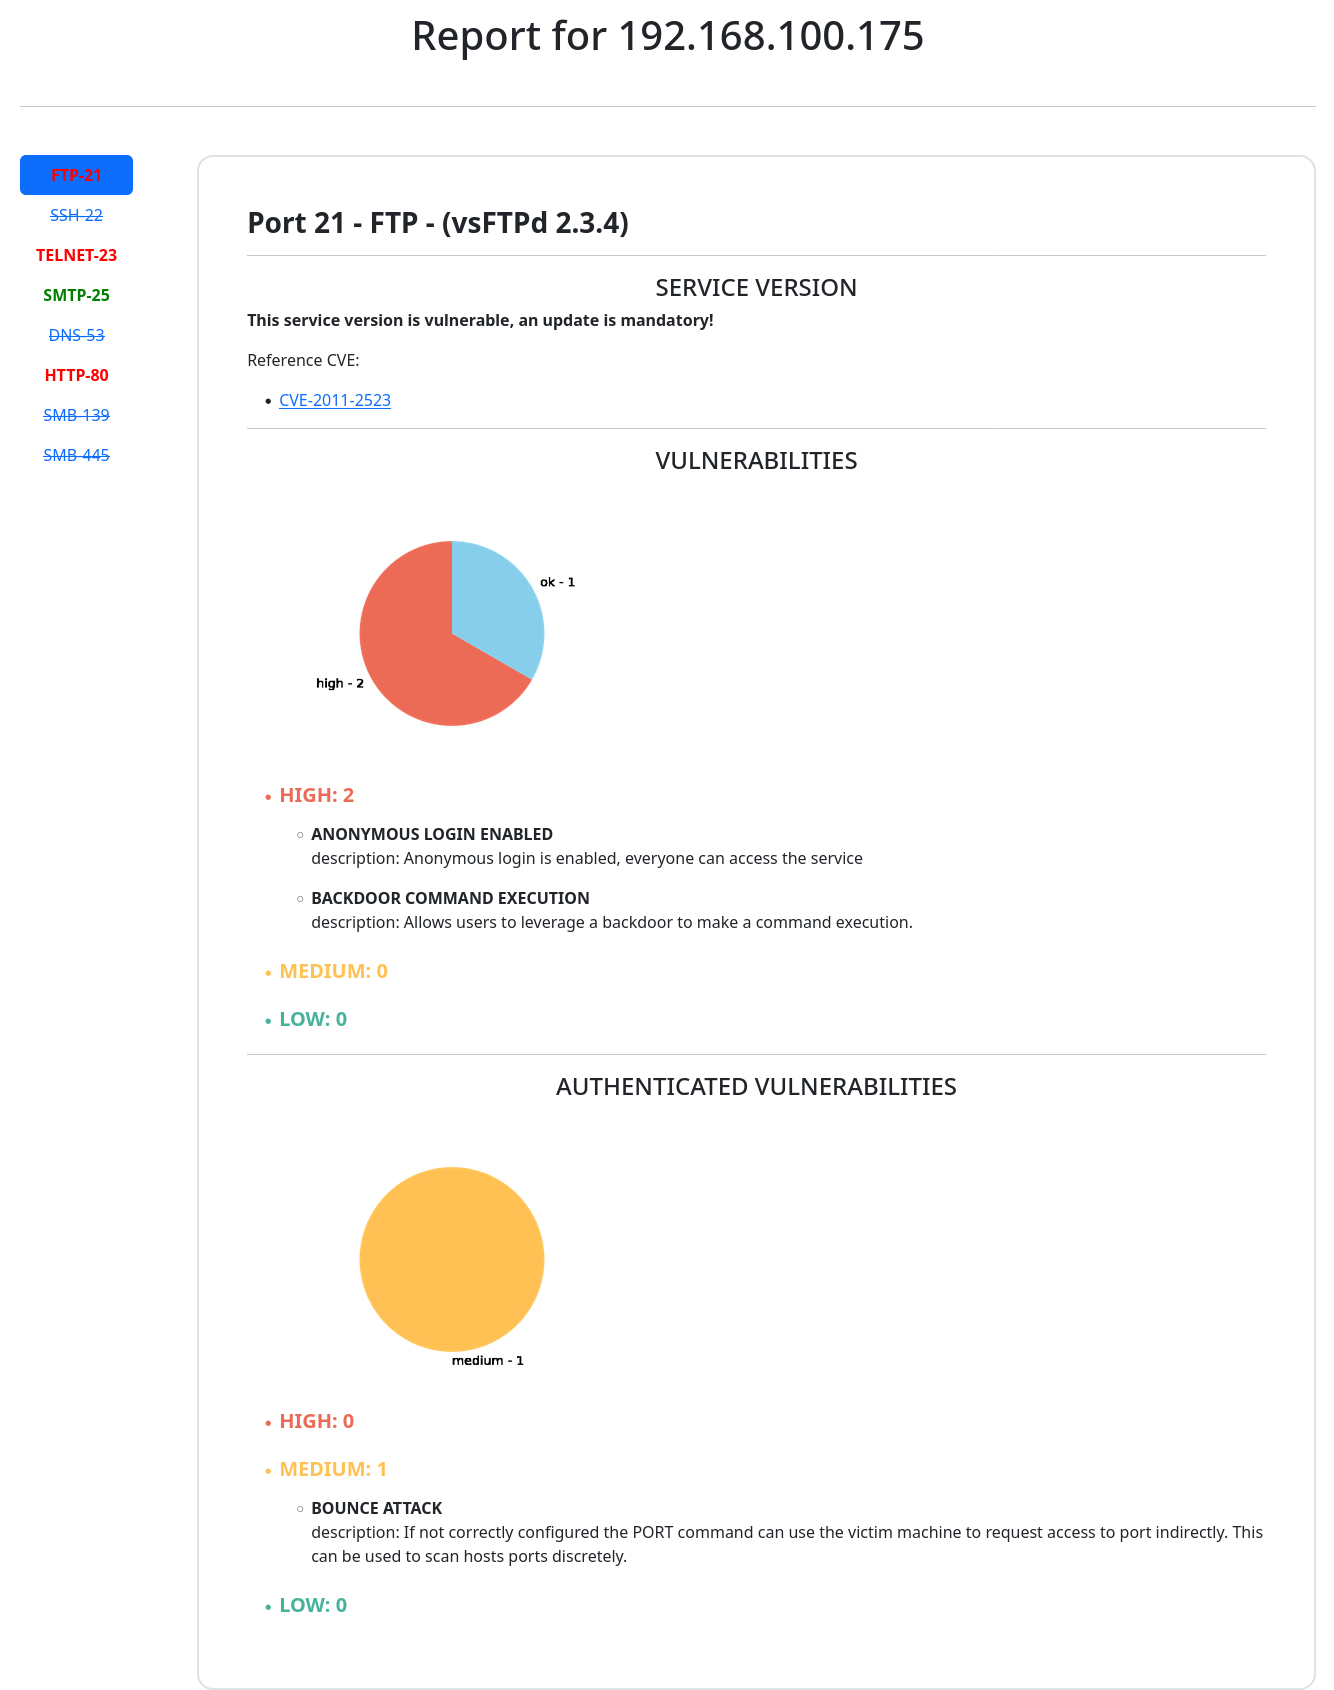
\includegraphics[width = 27em]{immagini/Res_html_vuln.png}
	\caption{Risultati del riconoscimento dei protocolli in formato HTML}
	\label{img:html_results}
\end{figure}
\noindent
Il risultato HTML è utilizzato per esprimere i dati del report in modo semplice e visivo. In questo modo chi visiona i risultati ha più facilità ad orientarsi tra i dati e le informazioni. La pagina principale presenta come titolo l'IP della macchina scansionata e due sezioni sottostanti. La parte sinistra contiene dei bottoni che rappresentano tutti i protocolli individuati e le rispettive porte, colorati in base ai risultati dei test. Un bottone barrato significa che non sono stati trovati test da svolgere, un bottone rosso indica la presenza di vulnerabilità all'interno dei protocolli o dei servizi e infine il bottone verde indica che tramite i test svolti non sono state individuate problematiche. A seguito del click su un bottone, nella sezione più grande a destra vengono mostrati i risultati in dettaglio. Inizialmente viene dichiarata se la versione utilizzata dal servizio è vulnerabile e successivamente, se presente, un'indicazione sul protocollo SSL/TLS utilizzato. La parte finale dei risultati riguarda le vulnerabilità scovate tramite i test. Sono suddivise in \lstinline{VULNERABILITIES} e \lstinline{AUTHENTICATED VULNERABILITIES} ed entrambe presentano un grafico che descrive il numero e la gravità delle vulnerabilità trovate.

% 
%			CAPITOLO 8: Conclusione
% 

\chapter{Conclusioni}
\label{cap:conclusioni}

L'applicativo sviluppato è in grado di svolgere correttamente le principali funzionalità presenti in un qualsiasi vulnerability scanner. \'{E} in grado di riconoscere correttamente i servizi presenti sulle macchine di prova ed è anche capace di fornire un report dettagliato di vulnerabilità in seguito a test svolti sulle porte individuate. La modularità con cui è stato scritto il codice permette di ampliare in modo molto semplice le capacità dell'applicativo, permettendo aggiornamenti e miglioramenti in un tempo ridotto.

\section{Sviluppi futuri}

Per poter trasformare questo progetto in un vero e proprio software utilizzabile è necessario implementare nuove funzionalità e nuovi test. L'applicativo ora è in grado di riconoscere 12 tra i principali protocolli e servizi utilizzati nelle comunicazioni di tutti i giorni e riesce a svolgere test su una piccola parte di configurazioni e vulnerabilità. Nelle sezioni seguenti sono stati riportate delle idee per poter rendere questo applicativo sempre più completo e funzionale.

\subsection{Scrittura di test automatizzata}

La scrittura dei test per ora è svolta manualmente e può essere molto onerosa, in quanto è necessario ricercare nuove vulnerabilità e riportarle all'interno dei rispettivi file JSON. Per poter affrontare questo problema si potrebbe implementare uno scraper che analizza script e test di altri scanner, per poterli adattare successivamente in file JSON interpretabili dall'applicativo. In questo modo sarebbe possibile ridurre il tempo passato nella scrittura dei test, impiegando le forze sullo sviluppo di altre funzionalità.

\subsection{Ampliamento dei protocolli supportati}

I protocolli supportati fin ora sono un numero molto ridotto rispetto a quelli utilizzati da grandi infrastrutture di rete. Sarebbe dunque opportuno implementare il riconoscimento di altri protocolli, in modo tale da poter svolgere un vulnerability scan più dettagliato e completo. Grazie alla modularità del codice questo problema è facilmente risolvibile, in quanto basterà implementare nuove funzioni di riconoscimento utilizzando un template già presente nel codice. Inserendo il nome della funzione all'interno di una lista specifica, questa verrà eseguita insieme a tutte le altre funzioni per lo scan di protocolli e servizi.

\subsection{Scansione di più host contemporaneamente}

L'applicativo nello stato attuale permette la scansione di un solo host alla volta. Una soluzione potrebbe essere quella di implementare un'analisi parallela di più dispositivi nella rete. In questo modo è possibile far partire un'unica scansione, senza ulteriori interventi umani, in modo tale da poter coprire l'intera infrastruttura di un'azienda. Per implementare ciò è possibile utilizzare i thread che, lavorando in parallelo sulle stesse operazioni, ma su host diversi, possono velocizzare di molto la verifica degli host e il riconoscimento dei protocolli.

\subsection{Esecuzione automatica e periodica}

Il programma creato è altamente dipendente dall'uomo, in quanto è necessario richiamarlo da linea di comando ogni volta che si vuole eseguire una scansione. Per ovviare a questo problema sarebbe possibile 
sviluppare uno script che richiama periodicamente l'applicativo per eseguire gli scan, in modo tale da verificare lo stato della rete di giorno in giorno o di settimana in settimana. Un'ulteriore funzionalità potrebbe essere quella di avvisare tramite mail o messaggio l'amministratore di rete ogni qual volta vengano rilevate nuove vulnerabilità sulle macchine. Essendo l'applicativo scritto in python, l'implementazione di questa funzionalità potrebbe essere fatta in modo molto semplice. 

\subsection{Evasione dei firewall}

Un'infrastruttura di rete a livello aziendale presenta sicuramente un firewall per la difesa della rete. Questo può essere un ostacolo per l'applicativo, poiché alcuni pacchetti potrebbero essere bloccati per via di alcune regole applicate. Di conseguenza è possibile implementare delle metodologie aggiuntive che permettano l'evasione dei filtri, in modo tale da poter svolgere uno scan senza troppe problematiche e allo stesso tempo verificare anche l'efficacia del firewall stesso. Per fare ciò è possibile implementare una nuova modalità di invio di pacchetti, in modo da renderli più discreti e difficilmente individuabili dagli strumenti di difesa.

%
%			BIBLIOGRAFIA
%

% Si può specificare a che livello della TOC deve essere la bibliografia.
% Il default è 'chapter', per 'part' usare
% \beforebibliography[part]
\beforebibliography
\bibliographystyle{unsrt}
\bibliography{bibliografia}

% 
%			APPENDICE A: Codice
% 
\appendix
\chapter{Codice}

All'interno della seguente appendice sono riportate parti di codice. Anche in questo caso alcune funzioni non verranno riportate per intero perché troppo complesse o per via di ripetizioni (per esempio verrà mostrata solo una funzione per il riconoscimento dei protocolli dato che le altre sono molto simili tra loro).
Il codice completo è visionabile sulla mia repository personale al link \url{ https://github.com/Veronica-Falgiani/Network-Protocol-Verification-Agent}

\section{main.py}
\begin{lstlisting}[language=Python, caption=, basicstyle=\ttfamily\scriptsize]
#!/bin/python3

# Imports
import os
import sys
from utils.parser import args_parse, ip_parse, port_parse
from utils.terminal_colors import print_ok, print_fail, print_cmd
from agent.host_scan import host_scan
from agent.port_scan import PortScan
from agent.service_scan import ServiceScan
from agent.execute_tests import ExecuteTests
from utils.write_result import write_result

if __name__ == "__main__":
    if "SUDO_UID" not in os.environ:
        print_fail("This program requires sudo privileges")
        sys.exit()

    # Get arguments from cmd line
    args = args_parse()

    host_arg = args.host_scan
    port_arg = args.port_scan
    ip = args.host
    ports_str = args.ports
    verbose = args.verbose
    no_tests = args.no_tests

    # Verify that user input is correct
    ip_parse(ip)
    ports_list = port_parse(ports_str)

    # Host scan
    print("--- Checking host ---")
    if host_scan(host_arg, ip, verbose):
        if verbose:
            print_ok("Host is up\n")
    else:
        if verbose:
            print_fail("Host is down\n")
        sys.exit()

    # Port scan
    print("--- Checking ports ---")
    port_scan = PortScan(ip)
    port_scan.port_scan(port_arg, ports_list, verbose)
    port_scan.get_open_ports()
    print_cmd(port_scan, verbose)

    # Protocol - Service scan
    print("--- Checking protocols and services ---")
    service_scan = ServiceScan(ip)
    if port_scan.type == "TCP":
        service_scan.tcp_scan(port_scan.open_ports, verbose)
    else:
        service_scan.udp_scan(port_scan.open_ports, verbose)
    if not no_tests:
        print_cmd(service_scan, verbose)

    # If the user has requested a simple scan, prints the results and interrupts the execution
    if no_tests:
        print(service_scan)
        sys.exit()

    # Testing all protocols
    print("--- Testing protocols and services ---")
    report = ExecuteTests(ip)
    report.execute_tests(service_scan.services, verbose)
    print("\n------------- RESULTS -------------")
    print(report)

    # Write to file results
    write_result(report)
\end{lstlisting}

\section{agent/}

\noindent
\textbf{host\_scan.py}
\\\\
Viene riportata solamente la funzione TCP\_SYN scan dato che le altre sono molto simili nei contenuti.
\begin{lstlisting}[language=Python, caption=, basicstyle=\ttfamily\scriptsize]
import sys
from utils.terminal_colors import print_fail, verbose_print
from scapy.all import *

# Ports used for syn and ack scan
SCAN_PORTS = [21, 22, 80, 443]


# Selecting the right scan based on the user input
def host_scan(host_arg: str, ip: str, verbose: bool):
    if verbose:
        verbose_print(f"Verifying {ip}")

    match host_arg:
        case "p":
            res_status = ping_scan(ip)
        case "s":
            res_status = tcp_syn_scan(ip)
        case "a":
            res_status = tcp_ack_scan(ip)
        case "u":
            res_status = udp_scan(ip)
        case None:
            res_status = ping_scan(ip)
        case _:
            print_fail("Cannot find host scan type")
            sys.exit()

    # Clean line
    print("\033[K", end="\r")

    return res_status


... <codice omesso> ...


# --------------------------
# TCP SYN
# --------------------------
def tcp_syn_scan(ip: str) -> bool:
    res_status = False

    for port in SCAN_PORTS:
        packet = IP(dst=ip) / TCP(dport=port, flags="S")
        res = sr1(packet, timeout=2, verbose=0)

        if res is not None:
            flag_res = res.sprintf("%TCP.flags%")

            if flag_res == "SA":
                res_status = True

    return res_status

... <codice omesso> ...
\end{lstlisting}

\newpage
\noindent
\textbf{port\_scan.py}
\\\\
Di seguito viene mostrato il codice in forma ridotta. Vengono riportate a titolo d'esempio le funzioni di scan Connect e TCP\_SYN 
\begin{lstlisting}[language=Python, caption=, basicstyle=\ttfamily\scriptsize]
import socket
import sys
from utils.terminal_colors import print_fail, print_warning, verbose_print
from scapy.all import *


class PortScan:
    def __init__(self, ip: str):
        self.ip = ip
        self.ports = {}
        self.type = ""
        self.open_ports = []

    def __str__(self):
        string = f"{'PORT':<10s} {'STATUS':<15s}\n"

        for key, value in self.ports.items():
            string += f"{str(key):<10s} {value:<15s}\n"

        return string

    def get_open_ports(self):
        for key, value in self.ports.items():
            if value != "closed" or value != "filtered":
                self.open_ports.append(key)

    # Selecting the right scan based on the user input
    def port_scan(self, port_arg: str, ports_list: list, verbose: bool):
        match port_arg:
            case "c":
                self.tcp_connect_scan(ports_list, verbose)
            case "s":
                self.tcp_syn_scan(ports_list, verbose)
            case "f":
                self.tcp_fin_scan(ports_list, verbose)
            case "n":
                self.tcp_null_scan(ports_list, verbose)
            case "x":
                self.tcp_xmas_scan(ports_list, verbose)
            case "u":
                self.udp_scan(ports_list, verbose)
            case None:
                self.tcp_connect_scan(ports_list, verbose)
            case _:
                print_fail("Cannot find scan type")
                sys.exit()

        # Clean line
        print("\033[K", end="\r")

        if len(self.ports) == 0:
            print_fail("No open ports found!")
            sys.exit()

    # Send: connect() (TCP with SYN)
    # Rec:  TCP with SYN/ACK -> open
    #       no response -> closed/filtered
    def tcp_connect_scan(self, ports_list: list, verbose: bool):
        self.type = "TCP"

        for port in ports_list:
            if verbose:
                print("\033[K", end="\r")
                verbose_print(f"Testing {port}")

            s = socket.socket(socket.AF_INET, socket.SOCK_STREAM)
            s.settimeout(3)
            res = s.connect_ex((self.ip, port))

            # Port open
            if res == 0:
                # print(f"{port} \t open")
                self.ports[port] = "open"

            # Port closed/filtered
            else:
                pass
                # print(f"{port} \t closed/filtered")
                # found_ports[port] = "closed/filtered"

            s.close()

    # Send: SYN
    # Rec:  SYN/ACK -> RST -> open
    #       RST ->  closed
    #       no response/ICMP unreachable -> filtered
    def tcp_syn_scan(self, ports_list: list, verbose: bool):
        self.type = "TCP"

        for port in ports_list:
            if verbose:
                print("\033[K", end="\r")
                verbose_print(f"Testing {port}")

            packet = IP(dst=self.ip) / TCP(dport=port, flags="S")
            res = sr1(packet, timeout=3, verbose=0)

            if res is None or (
                res.sprintf("%ICMP.type%") == 3
                and res.sprintf("%ICMP.code%") in [1, 2, 3, 9, 10, 13]
            ):
                # print(f"{port} \t filtered")
                self.ports[port] = "filtered"

            else:
                flag_res = res.sprintf("%TCP.flags%")

                if flag_res == "RA":
                    pass
                    # print(f"{port} \t closed")
                    # found_ports[port] = "closed"
                elif flag_res == "SA":
                    # print(f"{port} \t open")
                    self.ports[port] = "open"

    ... <codice omesso> ...
\end{lstlisting}

\newpage
\noindent
\textbf{service\_scan.py}
\\\\
Nel seguente codice sono riportate solo le funzioni per riconoscere FTP e FTPS. Il contenuto è stato ridotto per via della lunghezza eccessiva del file.
\begin{lstlisting}[language=Python, caption=, basicstyle=\ttfamily\scriptsize]
import socket
from time import sleep
from utils.terminal_colors import verbose_print
from scapy.all import *
from urllib.parse import urlparse
from http.client import HTTPConnection, HTTPSConnection
from ftplib import FTP, FTP_TLS
from smtplib import SMTP, SMTP_SSL
from telnetlib import Telnet
import ssl
import certifi
import dns.message, dns.query
from poplib import POP3, POP3_SSL
from imaplib import IMAP4, IMAP4_SSL
from impacket.smbconnection import SMBConnection
import paho.mqtt.client as mqtt_client
from operator import itemgetter
from enum import *
import subprocess


class ServiceScan:
    # Defining self signed certificate for tls/ssl
    context = ssl._create_unverified_context(ssl.PROTOCOL_TLS_CLIENT)
    context.options &= ~ssl.OP_NO_SSLv3
    context.minimum_version = 768
    context.load_verify_locations(certifi.where())

    def __init__(self, ip: str):
        self.ip = ip
        self.services = []

    def __str__(self):
        string = f"{'PORT':<10s} {'PROTOCOL':<15s} {'SERVICE':<100s}\n"

        for service in self.services:
            string += f"{str(service['port']):<10s} {service['protocol']:<15s} {service['service']:<100s}\n"

        return string

    def test_scan(self, open_ports: list, verbose: bool):
        # Write portocols to test here
        for self.check in self.tcp_check:
            self.check(self, open_ports, verbose)

        # Clean line for verbose print
        print("\033[K", end="\r")

        # Sorts list by port
        self.services = sorted(self.services, key=itemgetter("port"))

    def tcp_scan(self, open_ports: list, verbose: bool):
        for self.check in self.tcp_check:
            self.check(self, open_ports, verbose)

        # Out of for because I needed third argument
        self.nfs_check(open_ports, verbose, "T")

        # Clean line for verbose print
        print("\033[K", end="\r")

        # Sorts list by port
        self.services = sorted(self.services, key=itemgetter("port"))

    def udp_scan(self, open_ports: list, verbose: bool):
        for self.check in self.udp_check:
            self.check(self, open_ports, verbose)

        # Out of for because I needed third argument
        self.nfs_check(open_ports, verbose, "U")

        # Clean line for verbose print
        print("\033[K", end="\r")

        # Sorts list by port
        self.services = sorted(self.services, key=itemgetter("port"))

    # --------------------------
    # FTP
    # --------------------------
    def ftp_check(self, open_ports: list, verbose: bool):
        rem_ports = []
        ip = self.ip

        for port in open_ports:
            service = {}

            if verbose:
                print("\033[K", end="\r")
                verbose_print(f"Scanning {port} for FTP")

            try:
                ftp = FTP()
                ftp.connect(host=ip, port=port, timeout=3)
                ftp.quit()

                # smtp also responds to this, so we need to verify the banner
                s = socket.socket()
                s.connect((ip, port))
                banner = s.recv(1024)
                banner = banner.decode("utf-8", errors="ignore")

                if "FTP" in banner:
                    rem_ports.append(port)

                    service["port"] = port
                    service["protocol"] = "FTP"
                    service["service"] = str(banner).strip()[4:]

                    self.services.append(service)

                s.close()

            except Exception as e:
                pass

        for port in rem_ports:
            open_ports.remove(port)

    # --------------------------
    # FTP/SSL
    # --------------------------
    def ftps_check(self, open_ports: list, verbose: bool):
        rem_ports = []
        ip = self.ip

        for port in open_ports:
            service = {}

            if verbose:
                print("\033[K", end="\r")
                verbose_print(f"Scanning {port} for FTP-SSL")

            try:
                # FTP_SSL not properly working, need to find out why
                # ftps = FTP_TLS()
                # ftps.connect(ip, port, timeout=3)
                # banner = ftps.getwelcome()
                # ftps.quit()

                # smtp also responds to this, so we need to verify the banner ?
                sock = socket.create_connection((ip, port), timeout=3)
                ssock = ServiceScan.context.wrap_socket(sock, server_hostname=ip)
                ssl_version = ssock.version()

                sleep(1)  # Banner was cut in half so we need ot wait
                banner = ssock.recv(2048)
                banner = banner.decode("utf-8", errors="ignore")

                if "FTP" in banner:
                    rem_ports.append(port)

                    service["port"] = port
                    service["protocol"] = "FTP-SSL"
                    service["service"] = str(banner).strip()[4:] + " - " + ssl_version

                    self.services.append(service)

                ssock.close()

            except ssl.SSLCertVerificationError as e:
                print(port, e)

            except Exception as e:
                pass

        for port in rem_ports:
            open_ports.remove(port)

    ... <codice omesso> ...
    
    # --------------------------
    # UNDEFINED
    # --------------------------
    def undefined(self, open_ports: list, verbose: bool):
        rem_ports = []
        ip = self.ip

        for port in open_ports:
            service = {}

            if verbose:
                print("\033[K", end="\r")
                verbose_print(f"Scanning {port} for SSL-TLS")

            try:
                pass  # TODO
            except Exception as e:
                pass

        for port in rem_ports:
            open_ports.remove(port)

    # --------------------------
    # TEMPLATE
    # --------------------------
    def check(self, open_ports: list, verbose: bool):
        rem_ports = []
        ip = self.ip

        for port in open_ports:
            service = {}
            if verbose:
                print("\033[K", end="\r")
                verbose_print(f"Scanning {port} for PROTOCOL")

            try:
                # Insert code here

                rem_ports.append(port)
                service["port"] = port
                service["protocol"] = "MQTT"
                service["service"] = "undefined"

                self.services.append(service)

            except Exception:
                pass

        for port in rem_ports:
            open_ports.remove(port)

    # List of protocol scans to use
    tcp_check = [
        ftp_check,
        ssh_check,
        telnet_check,
        smtp_check,
        dns_check,
        http_check,
        pop_check,
        imap_check,
        smb_check,
        mqtt_check,
        # SSL protocols
        ftps_check,
        https_check,
        smtps_check,
        pops_check,
        imaps_check,
        mqtts_check,
        ssltls_check,
        # Undefined
        undefined,
    ]

    udp_check = [
        http_check,
        https_check,
        dns_check,
        # Undefined
        undefined,
    ]
\end{lstlisting}

\noindent
\textbf{results.py}
\begin{lstlisting}[language=Python, caption=, basicstyle=\ttfamily\scriptsize]
class Results:
    def __init__(self, port, prot, service):
        self.port = port
        self.prot = prot
        self.service = service
        self.prot_max_vulns = 0
        self.prot_max_auth_vulns = 0
        self.serv_max_vulns = 0
        self.serv_max_auth_vulns = 0
        self.found_vulns = []
        self.found_auth_vulns = []
        self.unsafe_ver = False
        self.unsafe_ver_cve = []
        self.unsafe_tls = False
        self.prot_auth = False
        self.serv_auth = False

    def __str__(self):
        string = f"{str(self.port):<10s} {self.prot:<15s} {self.service:<100s}\n|\n"

        # Print if the service version is vulnerable
        string += "| --------------- VERSION CHECK ---------------\n"
        if self.unsafe_ver:
            string += (
                "|\\___ THIS SERVICE VERSION IS VULNERABLE AND NEEDS TO BE UPDATED!\n"
            )
            string += "|     reference:\n"
            for cve in self.unsafe_ver_cve:
                cve_number = cve.split("?id=")[1]
                string += f"|     - {cve_number}: {cve}\n"

            string += "|\n"
        else:
            string += "|\\___ The service version is not vulnerable.\n|\n"

        # Print if the ssl/tls version is outdated
        if "TLS" in self.service or "SSL" in self.service:
            string += "| --------------- SSL/TLS CHECK ---------------\n"
            if self.unsafe_tls:
                string += "|\\___ THE SERVICE USES A DEPRECATED SSL/TLS PROTOCOL! \n|\n"
            else:
                string += "|\\___ The service uses the currently supported SSL/TLS protocol  \n|\n"

        # Print all the information about the tests
        string += "| --------------- VULNERABILITIES ---------------\n"
        if (self.prot_max_vulns + self.serv_max_vulns) == 0:
            string += "|\\___ No tests found for this protocol\n"
        elif len(self.found_vulns) == 0:
            string += "|\\___ The protocol has been tested and no vulnearbilities have been found\n"
        else:
            for vuln in self.found_vulns:
                string += f"|\\___ {vuln['name']}\n"
                string += f"|     description: {vuln['description']}\n"
                string += f"|     severity: {vuln['severity']}\n"

        string += (
            "|\n| --------------- AUTHENTICATED VULNERABILITIES ---------------\n"
        )
        if (self.prot_max_auth_vulns + self.serv_max_auth_vulns) == 0:
            string += "|\\___ No tests found for this protocol\n"
        elif not self.prot_auth and not self.serv_auth:
            string += "|\\___ No credentials were given\n"
        elif len(self.found_auth_vulns) == 0:
            string += "|\\___ The protocol has been tested and no vulnerabilities have been found\n"
        else:
            for vuln in self.found_auth_vulns:
                string += f"|\\___ {vuln['name']}\n"
                string += f"|     description: {vuln['description']}\n"
                string += f"|     severity: {vuln['severity']}\n"

        string += "\n\n"

        return string

    def __json__(self):
        repr = {
            "port": self.port,
            "protocol": self.prot,
            "service": self.service,
            "unsafe_version": self.unsafe_ver,
            "unsafe_version_cve": self.unsafe_ver_cve,
            "vulnerabilities": self.found_vulns,
            "auth_vulnerabilities": self.found_auth_vulns,
        }

        if "SSL" in self.service or "TLS" in self.service:
            position = list(repr.keys()).index('misconfigurations')
            items = list(repr.items())
            items.insert(position, ("unsafe_tls", self.unsafe_tls))
            repr = dict(items)

        return repr

    def add_prot_max(self, prot_max_vulns: int, prot_max_auth_vulns: int):
        self.prot_max_vulns = prot_max_vulns
        self.prot_max_auth_vulns = prot_max_auth_vulns

    def add_serv_max(self, serv_max_vulns: int, serv_max_auth_vulns: int):
        self.serv_max_vulns = serv_max_vulns
        self.serv_max_auth_vulns = serv_max_auth_vulns

    def set_vulns(self, vulns: dict):
        self.found_vulns.append(vulns)

    def set_auth_vulns(self, vulns: dict):
        self.found_auth_vulns.append(vulns)
\end{lstlisting}

\noindent
\textbf{execute\_tests.py}
\\\\
Viene riportato solo il codice che svolge i test sui protocolli, dato che le funzioni utilizzate per il test dei servizi sono identiche. Anche \lstinline{test_ssl()} è stato omesso per via della somiglianza con \lstinline{test()} 
\begin{lstlisting}[language=Python, caption=, basicstyle=\ttfamily\scriptsize]
import json
import os
import socket
import ssl
import certifi
import getpass
import re
from utils.terminal_colors import verbose_print
from agent.results import Results


class ExecuteTests:
    # Defining self signed certificate for tls/ssl
    context = ssl._create_unverified_context(ssl.PROTOCOL_TLS_CLIENT)
    context.options &= ~ssl.OP_NO_SSLv3
    context.minimum_version = 768
    context.load_verify_locations(certifi.where())

    def __init__(self, ip):
        self.ip = ip
        self.report = []

    def __str__(self):
        string = f"{'PORT':<10s} {'PROTOCOL':<15s} {'SERVICE':<100s}\n"

        for result in self.report:
            string += str(result) + "\n"

        return string

    def execute_tests(self, services: list, verbose: bool):
        # Protocol test
        for service in services:
            port = service["port"]
            prot = service["protocol"]
            service = service["service"]

            # Tests the generic protocol
            base_dir = os.path.dirname(__file__)
            rel_path_prot = "../tests/prot/" + prot.lower() + "_test.json"
            path_prot = os.path.join(base_dir, rel_path_prot)

            try:
                with open(path_prot) as file:
                    test_file = json.load(file)
                    vulns = test_file["vulns"]
                    login = test_file["login"]
                    auth_vulns = test_file["auth_vulns"]
                    serv_names = test_file["serv_names"]

                    # Create class
                    results = Results(port, prot, service)

                    prot_max_vulns = len(vulns)
                    i_mis = 1

                    prot_max_auth_vulns = len(auth_vulns)
                    i_auth = 1

                    results.add_prot_max(prot_max_vulns, prot_max_auth_vulns)

                    # Start testing for misconfigurations
                    auth = False
                    self.check_vulns(
                        vulns,
                        verbose,
                        i_mis,
                        prot_max_vulns,
                        port,
                        prot,
                        service,
                        results,
                        auth,
                    )

                    # If auth_vulns has tests, asks the user for login info and inserts the correct login messages in a list
                    if auth_vulns:
                        print("\n--- Asking for protocols credentials ---")

                        login_list = self.try_login(prot, port, service, login)

                        # Start testing for misconfigurations
                        if login_list:
                            results.prot_auth = True
                            auth = True
                            self.check_vulns(
                                auth_vulns,
                                verbose,
                                i_auth,
                                prot_max_auth_vulns,
                                port,
                                prot,
                                service,
                                results,
                                auth,
                                login_list,
                            )

                    # Services test
                    for name in serv_names:
                    
                        ... <codice omesso> ...

            except FileNotFoundError:
                results = Results(port, prot, service)

            self.report.append(results)

    def check_vulns(
        self,
        vulns,
        verbose,
        i_mis,
        max_vulns,
        port,
        prot,
        service,
        results,
        auth,
        login_list=[],
    ):
        for name, info in vulns.items():
            vuln = {}

            if verbose:
                print("\033[K", end="\r")
                verbose_print(
                    f"Scanning {port} with {prot} - {service} using {name} [{i_mis}/{max_vulns}]"
                )
                i_mis += 1

            # Complex ssl/tls test: establishes a connection and then sends a message and compares results
            if "SSL" in prot:
                vuln = self.test_ssl(name, info, self.ip, port, service, login_list)
                self.check_tls(service, results)

            # Complex test: sends a message and compares the results
            elif "recv" in info or "not_recv" in info:
                vuln = self.test(name, info, self.ip, port, service, login_list)

            # Simple test: checks if the port is open
            else:
                vuln["name"] = name
                vuln["service"] = service
                vuln["description"] = info["description"]
                vuln["severity"] = info["severity"]

            if vuln and auth:
                results.set_auth_vulns(vuln)
            elif vuln and not auth:
                results.set_vulns(vuln)

            # Clean line
            print("\033[K", end="\r")

    def test(self, name: str, info: dict, ip: str, port: int, service: str, login_list):
        recv = None
        not_recv = None

        send_str = info["send"]
        send_list = send_str.split("~~")

        if "recv" in info:
            recv = info["recv"]
        elif "not_recv" in info:
            not_recv = info["not_recv"]

        try:
            sock = socket.socket(socket.AF_INET, socket.SOCK_STREAM)
            sock.settimeout(5)
            sock.connect((ip, port))

            for message in login_list:
                sock.send(message.encode())

            # Sends all the commands to the server
            for send in send_list:
                # print(send)
                sock.send(send.encode())
                res = sock.recv(1024)
                # print(res.decode())

            # Compares the received message to the one in the json
            if (
                recv is not None
                and re.search(recv, res.decode())
                or not_recv is not None
                and not re.search(not_recv, res.decode())
            ):
                vuln = {}
                vuln["name"] = name
                vuln["service"] = service
                vuln["description"] = info["description"]
                vuln["severity"] = info["severity"]
                return vuln

            sock.close()

        except TimeoutError:
            pass

    def test_ssl(
        self, name: str, info: dict, ip: str, port: int, service: str, login_list
    ):
            ... <codice omesso> ...
            
    def check_banner(self, service: str, vuln_serv_version: dict, results: Results):
        for version, cve in vuln_serv_version.items():
            if version in service:
                results.unsafe_ver = True
                results.unsafe_ver_cve = cve

    def check_tls(self, service: str, results: Results):
        if not ("TLSv1.3" in service or "TLSv1.2" in service):
            results.unsafe_tls = True

    def try_login(self, prot, port, service, login) -> list:
        # Asks the user max 3 times for the password
        for i in range(3):
            # Opens SSL socket
            if "SSL" in prot:
                sock = socket.create_connection((self.ip, port), timeout=3)
                sock = ExecuteTests.context.wrap_socket(sock, server_hostname=self.ip)

            # Opens simple socket
            else:
                sock = socket.socket(socket.AF_INET, socket.SOCK_STREAM)
                sock.settimeout(5)
                sock.connect((self.ip, port))

            # Asks the user for login ingo
            print(f"{prot} - {service} username: ", end="")
            username = input()
            password = getpass.getpass(f"{prot} - {service} password: ")
            if username == "" and password == "":
                login_list = []
                return login_list
            else:
                login_str = login["send_str"].replace("_username_", username)
                login_str = login_str.replace("_password_", password)

            # Sends the login strings to the server
            login_list = login_str.split("~~")
            for message in login_list:
                sock.send(message.encode())
                res = sock.recv(1024)

            # Checks the response of the server
            if re.search(login["recv_str"], res.decode()):
                sock.close()
                return login_list
            else:
                sock.close()
                print(f"Failed login {i + 1}/3")

        sock.close()
        login_list = []
        print("Max login failed")
        return login_list
\end{lstlisting}

\section{utils/}

\noindent
\textbf{parser.py}
\begin{lstlisting}[language=Python, caption=, basicstyle=\ttfamily\scriptsize]
import argparse
import sys
import socket
import re
from utils.terminal_colors import print_fail, print_warning

# python3 main.py -hs p -ps s 100:200 192.168.0.1


def args_parse():
    parser = argparse.ArgumentParser(
        prog="main.py",
        description="Agent for Advanced Network Protocol Verification. This program needs sudo privileges to run.",
        add_help=False,
        formatter_class=argparse.RawTextHelpFormatter,
    )

    parser.add_argument(
        "-h", "--help", action="help", help="Show this help message and exit"
    )
    parser.add_argument(
        "-v", "--verbose", action="store_true", help="Increase output verbosity"
    )
    parser.add_argument(
        "-nt",
        "--no_tests",
        action="store_true",
        help="Scans the target for services but doesn't execute a vulnerability scan",
    )
    parser.add_argument(
        "-hs",
        "--host_scan",
        help="Host scan to execute: [p]ing, [s]yn, [a]ck, [u]dp (ping scan will be used by default)",
    )
    parser.add_argument(
        "-ps",
        "--port_scan",
        help="Port scan to execute: [c]onnect, [s]yn, [f]in, [n]ull, [x]mas, [u]dp (connect scan will be used by default)",
    )
    parser.add_argument(
        "ports",
        help="Single port [x], multiple ports [x,y,z],  port range [x:y] to scan or all ports [all]",
    )
    parser.add_argument("host", help="Host to scan using ipv4 address")

    args = parser.parse_args()

    return args


# Parses ip from user input
def ip_parse(ip: str):
    regex = "^((25[0-5]|2[0-4][0-9]|1[0-9][0-9]|[1-9]?[0-9])\\.){3}(25[0-5]|2[0-4][0-9]|1[0-9][0-9]|[1-9]?[0-9])$"

    if ip == "localhost":
        ip = "127.0.0.1"
    if re.search(regex, ip):
        return
    else:
        print_fail("IP not valid!")
        sys.exit()


# Parsing ports we need to scan from user input
def port_parse(port_str: str) -> list:
    ports = []

    if port_str == "all":
        ports = list(range(0, 65536))

    # Contiguous port list
    elif ":" in port_str:
        p_range = port_str.split(":")

        if (
            p_range[0].isnumeric()
            and p_range[1].isnumeric()
            and int(p_range[0]) <= int(p_range[1])
            and 0 <= int(p_range[0]) <= 65535
            and 0 <= int(p_range[1]) <= 65535
        ):
            for i in range(int(p_range[0]), int(p_range[1]) + 1):
                ports.append(i)
        else:
            print_fail("Ports are not valid!")
            sys.exit()

    # Random port list
    elif "," in port_str:
        p_list = port_str.split(",")
        for item in p_list:
            if item.isnumeric() and int(item) >= 0 and int(item) <= 65535:
                ports.append(int(item))
            else:
                print_warning(f"port {item} not valid! Skipping it")

        if len(ports) == 0:
            print_fail("Ports are not valid!")
            sys.exit()

        ports.sort()

    # Single port
    elif port_str.isnumeric() and int(port_str) >= 0 and int(port_str) <= 65535:
        ports.append(int(port_str))

    # Generic error
    else:
        print_fail("Ports are not valid!")
        sys.exit()

    return ports
\end{lstlisting}

\noindent
\textbf{terminal\_colors.py}
\begin{lstlisting}[language=Python, caption=, basicstyle=\ttfamily\scriptsize]
class bcolors:
    HEADER = "\033[95m"
    OKBLUE = "\033[94m"
    OKCYAN = "\033[96m"
    OKGREEN = "\033[92m"
    WARNING = "\033[93m"
    FAIL = "\033[91m"
    ENDC = "\033[0m"
    BOLD = "\033[1m"
    UNDERLINE = "\033[4m"


# Green print
def print_ok(string: str):
    print(bcolors.OKGREEN + string + bcolors.ENDC)


# Yellow print
def print_warning(string: str):
    print(bcolors.WARNING + string + bcolors.ENDC)


# Red print
def print_fail(string: str):
    print(bcolors.FAIL + string + bcolors.ENDC)


# Cyan print
def verbose_print(string: str):
    print(bcolors.OKCYAN + string + bcolors.ENDC, end="\r")


def print_cmd(string, verbose):
    if verbose:
        print(string)
\end{lstlisting}

\noindent
\textbf{write\_results.py}
\\\\
La funzione utilizzata per creare il codice HTML è stata ridotta per via della lunghezza eccessiva e la semplicità del codice.
\begin{lstlisting}[language=Python, caption=, basicstyle=\ttfamily\scriptsize]
import os
from datetime import datetime
import matplotlib.pyplot as plt
import json
from jinja2 import Environment, FileSystemLoader
from agent.results import Results


TIME = "Result_" + datetime.today().strftime("%Y-%m-%d_%H:%M:%S")
RES_DIR = "res/" + TIME + "/"


def write_result(report: Results):
    # Creates directories for result files (if they don't exist)
    os.makedirs(os.path.dirname("res/"), exist_ok=True)
    os.makedirs(os.path.dirname(RES_DIR), exist_ok=True)
    os.makedirs(os.path.dirname(f"{RES_DIR}img/"), exist_ok=True)
    os.chmod("res/", 0o777)
    os.chmod(f"{RES_DIR}", 0o777)
    os.chmod(f"{RES_DIR}img/", 0o777)

    log_result(report)
    json_result(report)
    html_result(report)

    print(f"Results can be found in: {RES_DIR}")


# Writes a human readable log
def log_result(report):
    file_log = RES_DIR + f"{report.ip}_results.log"

    with open(file_log, "w") as res_file:
        res_file.write(f"##### RESULTS FOR {report.ip} #####\n\n")
        res_file.write("PORT \t PROTOCOL \t SERVICE\n")
        res_file.write("----------------------------\n\n\n")

        for result in report.report:
            res_file.write(str(result))


# Creates a json file with all the results
def json_result(report):
    file_json = RES_DIR + f"{report.ip}_results.json"

    with open(file_json, "w") as res_file:
        res_dict = {
            "ip": report.ip,
            "timestamp": datetime.today().strftime("%Y-%m-%d_%H:%M:%S"),
            "services": [],
        }

        for result in report.report:
            res_dict["services"].append(result.__json__())

        json.dump(res_dict, res_file, indent=4)


# Creates a html page with results and graphs
def html_result(report: Results):
    # Creates a directory (if it doesn't exist) and a result file
    file_html = RES_DIR + f"{report.ip}_results.html"

    html_pills = ""
    html_title = ""
    html_protocols = ""

    for result in report.report:
        html_version = ""
        html_tls = ""
        html_vulns = ""
        html_auth_vulns = ""

        # Protocol name and service version
        html_title = f"""
            <div id={result.prot}-{result.port} class="tab-pane fade">
                <h3><b>Port {result.port} - {result.prot} - {result.service}</b></h3>
        """

        ... <codice omesso> ...
        
        # Checks if there are vulns to print
        if (result.serv_max_vulns + result.prot_max_vulns) == 0:
            html_vulns += """
                <div class='my-3'>
                    <hr>
                    <h4 style="text-align:center"> VULNERABILITIES </h4>
                    <p class="my-3">No tests found for the protocol</p>
                </div>
            """

        # Checks if the protocol has vulns or not
        elif len(result.found_vulns) != 0:
            severity_html = {
                "high": 0,
                "high_results": "",
                "medium": 0,
                "medium_results": "",
                "low": 0,
                "low_results": "",
                "ok": 0,
            }

            html_vulns += f"""
                <div class='my-3'>
                    <hr>
                    <h4 style="text-align:center"> VULNERABILITIES </h4>
                    <img src="img/{result.prot}-{result.port}.png" width="400">
                    <ul>
            """

            for vuln in result.found_vulns:
                match vuln["severity"]:
                    case "high":
                        severity_html["high"] += 1
                        severity_html["high_results"] += f"""
                            <li class='my-3'><b> {vuln["name"]} </b><br> description: {vuln["description"]}</li> 
                        """

                    case "medium":
                        severity_html["medium"] += 1
                        severity_html["medium_results"] += f"""
                            <li class='my-3'><b> {vuln["name"]} </b><br> description: {vuln["description"]}</li> 
                        """

                    case "low":
                        severity_html["low"] += 1
                        severity_html["low_results"] += f"""
                            <li class='my-3'><b> {vuln["name"]} </b><br> description: {vuln["description"]}</li> 
                        """

            html_vulns += (
                f"<li style='color:#EC6B56'><h5><b> HIGH: {severity_html['high']} </b></h5></li>"
                + f"<ul class='mb-4'> {severity_html['high_results']}</ul>"
                + f"<li style='color:#FFC154'><h5><b> MEDIUM: {severity_html['medium']} </b></h5></li>"
                + f"<ul class='mb-4'>{severity_html['medium_results']}</ul>"
                + f"<li style='color:#47B39C'><h5><b> LOW: {severity_html['low']} </b></h5></li>"
                + f"<ul class='mb-4'> {severity_html['low_results']}</ul>"
                + "</ul></div>"
            )

            draw_graph(
                severity_html,
                result,
                (result.prot_max_vulns + result.serv_max_vulns),
                "",
            )

        # No vulns for the specified protocol
        else:
            html_vulns += """
                <div class='my-3'>
                    <hr>
                    <h4 style="text-align:center"> VULNERABILITIES </h4>
                    <p class="my-3">The service has been tested and no vulnerabilities have been found</p>
                </div>
            """
        
        ... <codice omesso> ...

        html_protocols += (
            html_title
            + html_version
            + html_tls
            + html_vulns
            + html_auth_vulns
            + "</div>"
        )

    # Setup html template via jinja2 and write to file
    env = Environment(loader=FileSystemLoader("utils"))
    template = env.get_template("report_template.html")

    html = template.render(
        page_title_text=f"Result {TIME}",
        title_text=f"Report for {report.ip}",
        html_pills=html_pills,
        html_protocols=html_protocols,
    )

    with open(file_html, "w") as res_file:
        res_file.write(html)


# Creates a png image of a pie chart based on the results of a protocol
def draw_graph(severity_html: dict, result: Results, max_vulns: int, type: str):
    labels = "high", "medium", "low", "ok"
    colors = ["#EC6B56", "#FFC154", "#47B39C", "skyblue"]

    severity_html["ok"] = (
        max_vulns
        - severity_html["high"]
        - severity_html["medium"]
        - severity_html["low"]
    )

    # Creating pie chart for html
    sizes = [
        severity_html["high"],
        severity_html["medium"],
        severity_html["low"],
        severity_html["ok"],
    ]

    wedges, texts = plt.pie(
        sizes,
        labels=labels,
        startangle=90,
        colors=colors,
        textprops={"color": "w", "size": "x-large"},
    )

    # Updates labels with counters and removes labels that correspond to 0 vulns
    for label in texts:
        label_txt = label.get_text()
        label.set_text(f"{label_txt} - {severity_html[label_txt]}")
        if label_txt != "ok" and severity_html[label_txt] == 0:
            label.set_text("")
        elif label_txt == "ok" and severity_html["ok"] == 0:
            label.set_text("")

    plt.savefig(
        f"{RES_DIR}/img/{result.prot}-{result.port}{type}.png", transparent=True
    )
    plt.clf()
\end{lstlisting}

\noindent
\textbf{report\_template.html}
\begin{lstlisting}[language=html, caption=, basicstyle=\ttfamily\scriptsize]
<html data-bs-theme="dark">
    <head>
        <title>{{page_title_text}}</title>
        <link href="https://cdn.jsdelivr.net/npm/bootstrap@5.3.5/dist/css/bootstrap.min.css" rel="stylesheet" integrity="sha384-SgOJa3DmI69IUzQ2PVdRZhwQ+dy64/BUtbMJw1MZ8t5HZApcHrRKUc4W0kG879m7" crossorigin="anonymous">
        <script src="https://cdn.jsdelivr.net/npm/bootstrap@5.3.5/dist/js/bootstrap.bundle.min.js" integrity="sha384-k6d4wzSIapyDyv1kpU366/PK5hCdSbCRGRCMv+eplOQJWyd1fbcAu9OCUj5zNLiq" crossorigin="anonymous"></script>
    </head>
    <body>
        <div class="container">
            <div class="mx-auto m-5">
                <h1 class="text-center">{{title_text}}</h1>
            </div>
            <hr>
            <div class="d-flex align-items-start mt-5">
                <div class="nav flex-column nav-pills me-3">
                    {{html_pills}}
                </div>
                <div class="container-sm tab-content ms-5 p-5 border border-2 rounded-4">
                    {{html_protocols}}
                </div>
            </div>
        </div>
    </body>
</html>
\end{lstlisting}

% 
%			APPENDICE B: Codice
% 

\chapter{Esempio file di test}
\label{cap:file_test}

I file di test riportati riguardano il protocollo FTP e il servizio vsFTPd. I contenuti dei JSON sono stati redatti a titolo d'esempio. Per tanto hanno ancora molte informazioni che possono essere aggiunte per svolgere in modo ancora più approfondito i test.
\\\\
\noindent
\textbf{Test per il protocollo FTP}
\\\\
Il seguente file presenta i test per le vulnerabilità più conosciute del protocollo FTP. Queste informazioni sono state recuperate tramite pagine di CVE e script già presenti per altri software.
\begin{lstlisting}[caption=, basicstyle=\ttfamily\footnotesize]
{
  "vulns": {
    "ANONYMOUS LOGIN ENABLED" :{
      "description": "Anonymous login is enabled, everyone can access the service",
      "send": "\n~~USER anonymous\n~~PASS\n",
      "recv": "230",
      "severity": "high"
    },
    "CVE-2010-1938": {
      "description": "Allows remote attackers to cause a denial of service (daemon crash) or possibly execute arbitrary code via a long username.",
      "send": "\n~~user AAAAAAAAAAAAAAAAAAAAAAAAAAAAAAAAAAAAAAA\n",
      "not_recv": "331 Please specify the password",
      "severity": "high"
    }
  },
  "login": {
    "send_str": "\n~~USER _username_\n~~PASS _password_\n",
    "recv_str": "230 Login successful."
  },
  "auth_vulns": {
    "BOUNCE ATTACK": {
      "description": "If not correctly configured the PORT command can use the victim machine to request access to port indirectly. This can be used to scan hosts ports discretely.",
      "send": "PORT\n",
      "not_recv": "500",
      "severity": "medium"
    }
  },
  "serv_names": [
    "vsftpd"
  ]
}
\end{lstlisting}

\noindent
\textbf{Test per il servizio vsFTPd}
\\\\
Il seguente file contiene un test di esempio per il servizio vsFTPd. Le informazioni per ricreare le vulnerabilità che colpiscono questo servizio sono molto complesse e difficili da riportare. Per questo anche altre piattaforme preferiscono individuare le vulnerabilità presenti dalla versione del servizio. 
\begin{lstlisting}[caption=, basicstyle=\ttfamily\footnotesize]
{
  "vulns": {
    "BACKDOOR COMMAND EXECUTION": {
      "description": "Allows users to leverage a backdoor to make a command execution.",
      "send": "\n~~USER X:)\n~~PASS X\n~~id\n",
      "not_recv": "530",
      "severity": "high"
    }
  },
  "login": {},
  "auth_vulns": {},
  "vuln_serv_version": {
    "1.1.3": ["https://www.cve.org/CVERecord?id=CVE-2004-0042"],
    "2.0.5": ["https://www.cve.org/CVERecord?id=CVE-2004-0042"],
    "2.3.4": ["https://www.cve.org/CVERecord?id=CVE-2011-2523"],
    "3.0.2": ["https://www.cve.org/CVERecord?id=CVE-2015-1419"]
  }
}
\end{lstlisting}


\end{document}
